%!TEX root=/home/ska124/Dropbox/Thesis/thes-full.tex
%%%%%%%%%%%%%%%%%%%%%%%%%%%%%%%%%%%%%%%%%%%%%%%%%%%%
%
%     Chapter 3   
%
%%%%%%%%%%%%%%%%%%%%%%%%%%%%%%%%%%%%%%%%%%%%%%%%%

\chapter{Amoeba Cache Architecture}
\label{chap:ac_architecture}

As described in Section \ref{sec:cache_memory_systems}, a conventional cache organises the data array into a 2 dimensional structure. A transparently addressed cache uses the same namespace (memory address space layout) as the main memory. The blocks which are stored in the sets are \textit{tagged} with the aligned start address of block present in the main memory. The \textit{tags} for the cache blocks currently present in the cache set are maintained in a separate array. When a search is being performed to find out whether a required physical address is present in the cache, the tag array is looked up to determine a cache hit or a cache miss. The organization of the cache set and tag array is shown in Figure \ref{fig:set_assoc_arch}. The effective address is the virtual address supplied by the CPU of the required datum. The component bits of the effective address is segmented into 3 parts which form the \textit{Virtual Page Number(VPN)}, set number and byte offset. The set number and byte offset are looked up in the tag array while the VPN is looked up in the \textit{Translation Lookaside Buffer(TLB)} to check that the current process has brought in the corresponding page and it is valid. The organisation described (and shown in Fig \ref{fig:set_assoc_arch}) is virtually indexed, physically tagged organisation where the lookup logic does not include the TLB translation in the critical path to enable faster searches. There are other organisations such as virtually indexed, virtually tagged and physically indexed, physically tagged which are uncommon due to inherent issues with their design. The tradeoff for a virtually indexed, physically tagged cache is that it can only grow in size with an increase in the associativity of each set, or an increase in the size of each cache block. The Intel Sandy Bridge architecture is known to use a virtually indexed, physically tagged cache organisation.



\begin{figure}[b]
  %% Pg 84 - Jacob
  \begin{center}
    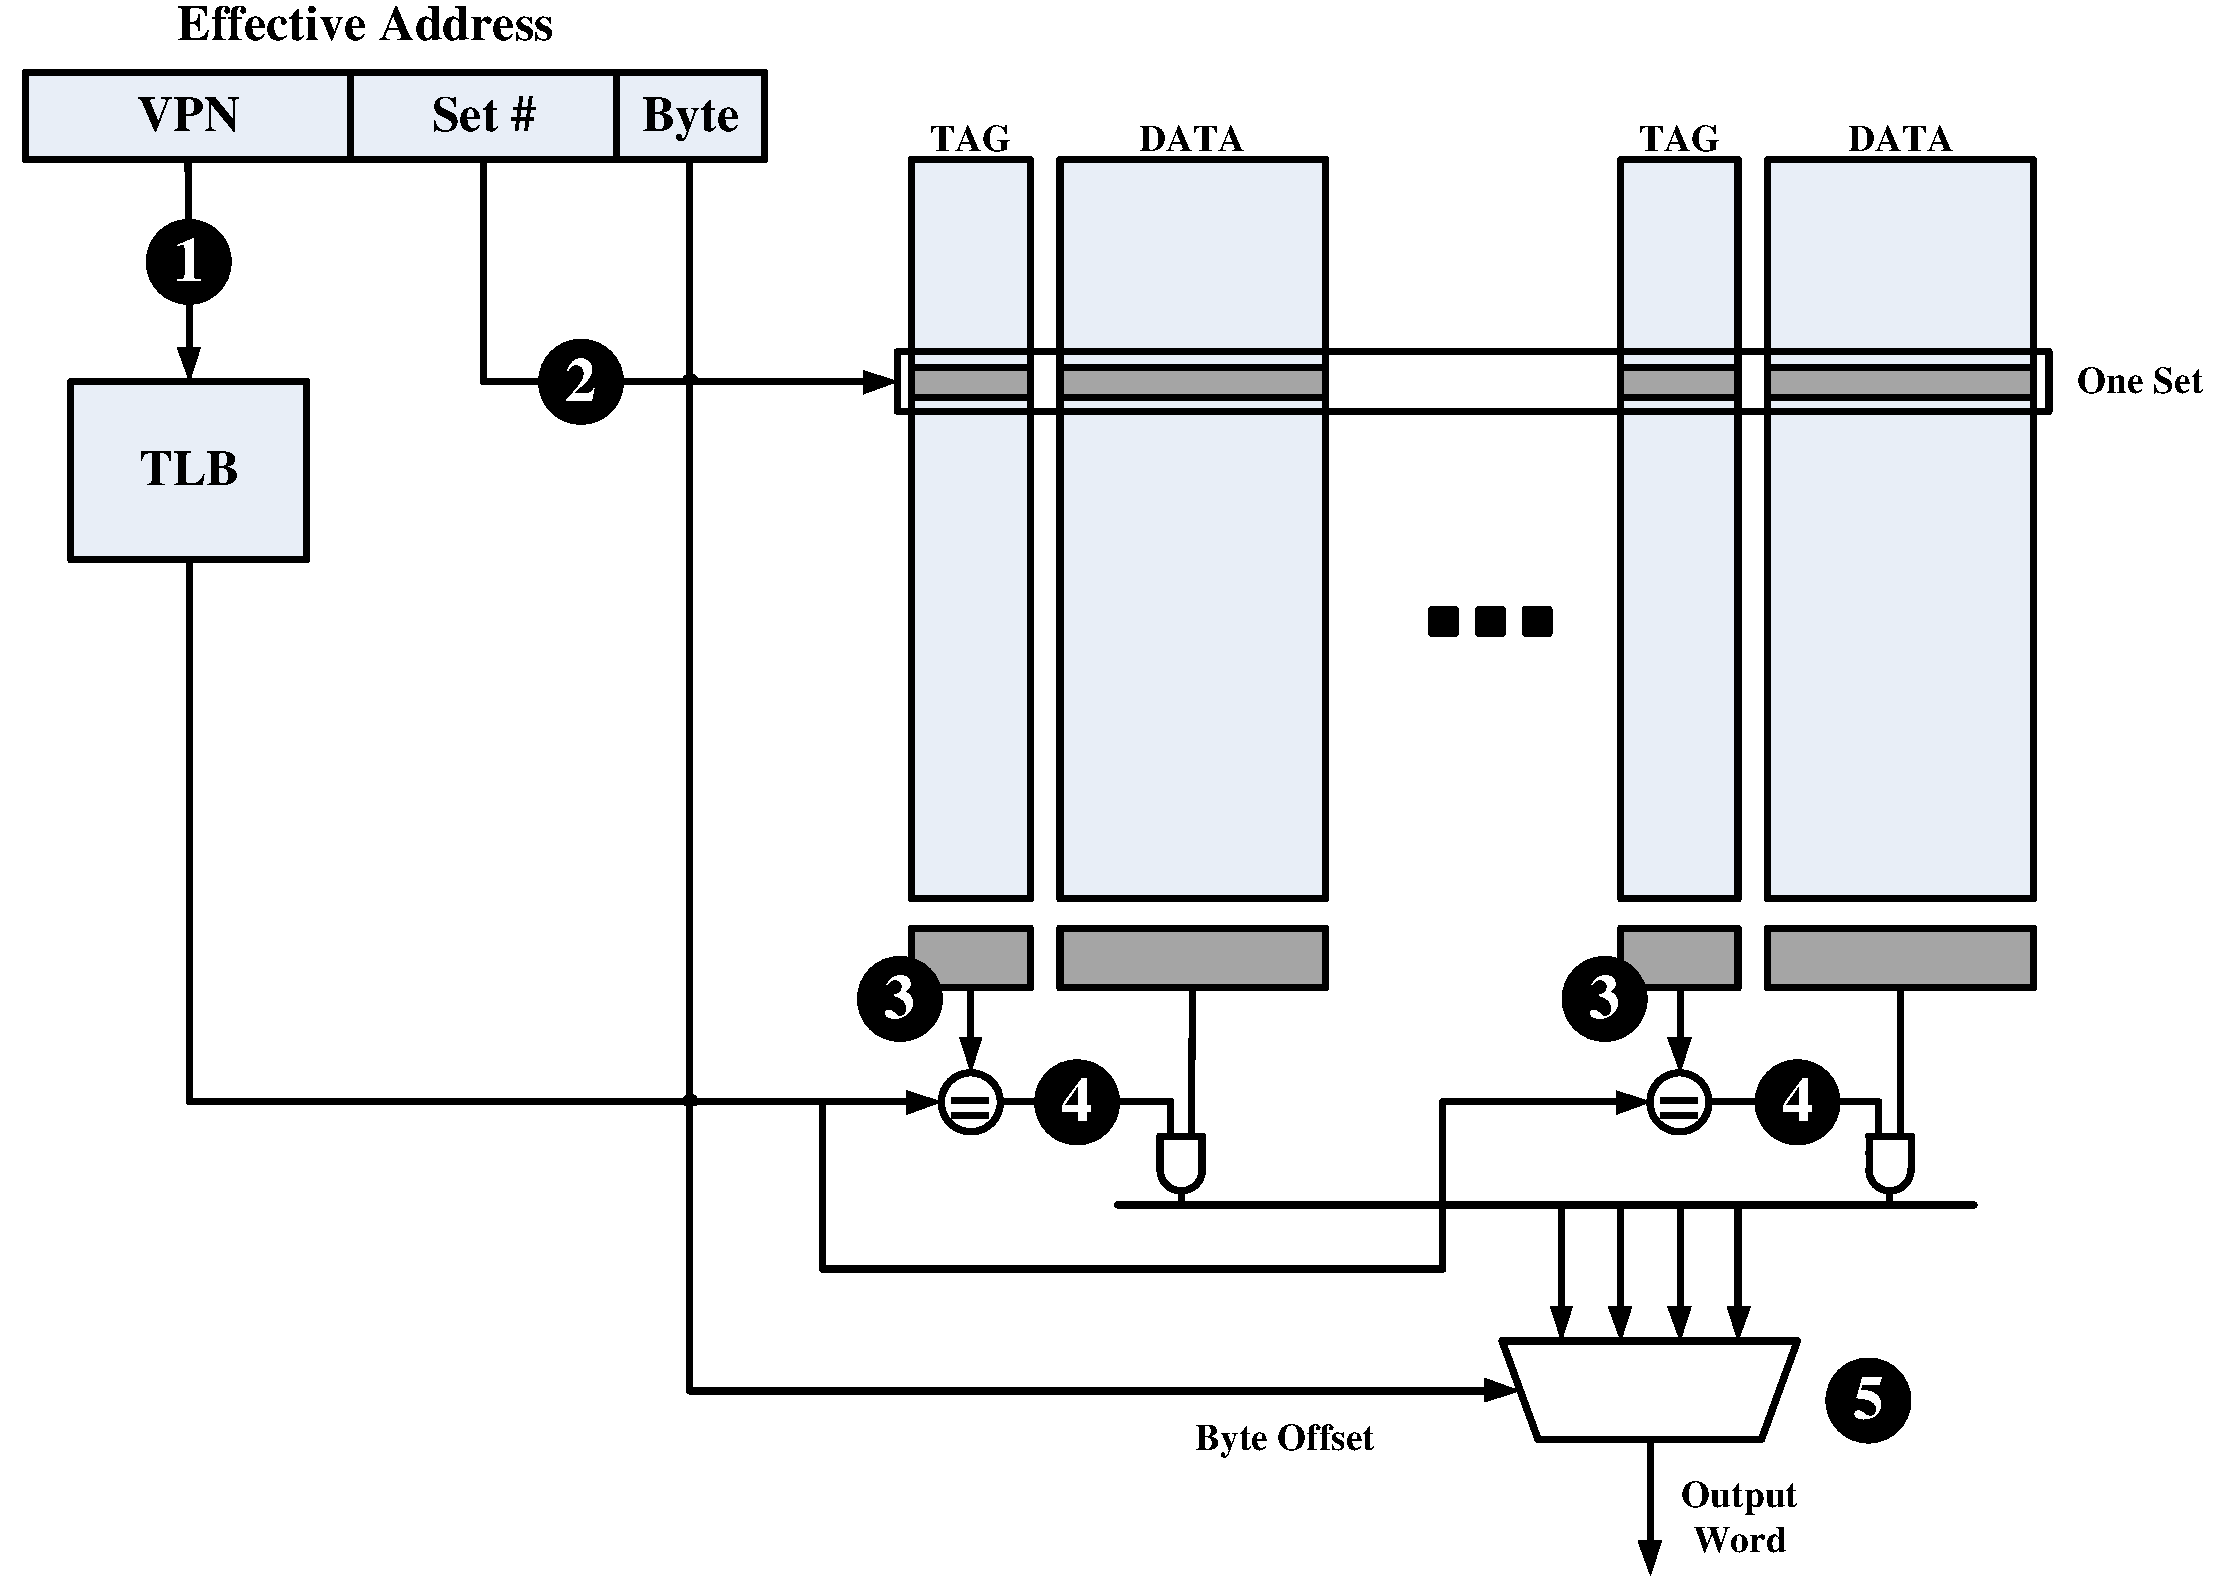
\includegraphics[width=\textwidth]{files/Figures/06-NWaySetAssocCache.pdf}
    \caption[Conventional N-Way Set-Associative Cache]{\textbf{Conventional N-Way Set-Associative Cache} \bigspot{1} The Virtual Page Number (VPN) is used to look up the entry in the Translation Lookaside Buffer (TLB) \bigspot{2} According to the number of sets in the cache, the following bits from the address are used to look up the corresponding set from the cache \bigspot{3} The tags read out from the set are compared with the translation from the TLB and tested for equality \bigspot{4} The corresponding cache block is forwarded to the output buffer for the tag which matches the TLB lookup \bigspot{5} Using the byte offset from the CPU, the mutiplexer selects the correponding critical word }
    \label{fig:set_assoc_arch}
  \end{center}
\end{figure}

\clearpage

In contrast to a conventional cache, the \AC\ architecture enables the memory hierarchy to fetch and allocate space for a range of words (i.e. a variable granularity cache block) based on the spatial locality of the application. For example, consider a 64K cache (256 sets) that allocates 256 bytes per set. These 256 bytes can adapt to support, for example, eight 32-bytes blocks, thirty-two 8-byte blocks, or four 32-byte blocks and sixteen 8-byte blocks, based on the set of contiguous words likely to be accessed. 
\\ \\
The key challenges to realising the \AC\ architecture are
\begin{enumerate}[noitemsep]
	\item To support a variable number of blocks per set
	\item To support a variable granularity for each block
	\item To support a variable number of tags, which correspond to the blocks in the set
\end{enumerate}

\begin{figure}[h]
  %% Pg 84 - Jacob
  \begin{center}
    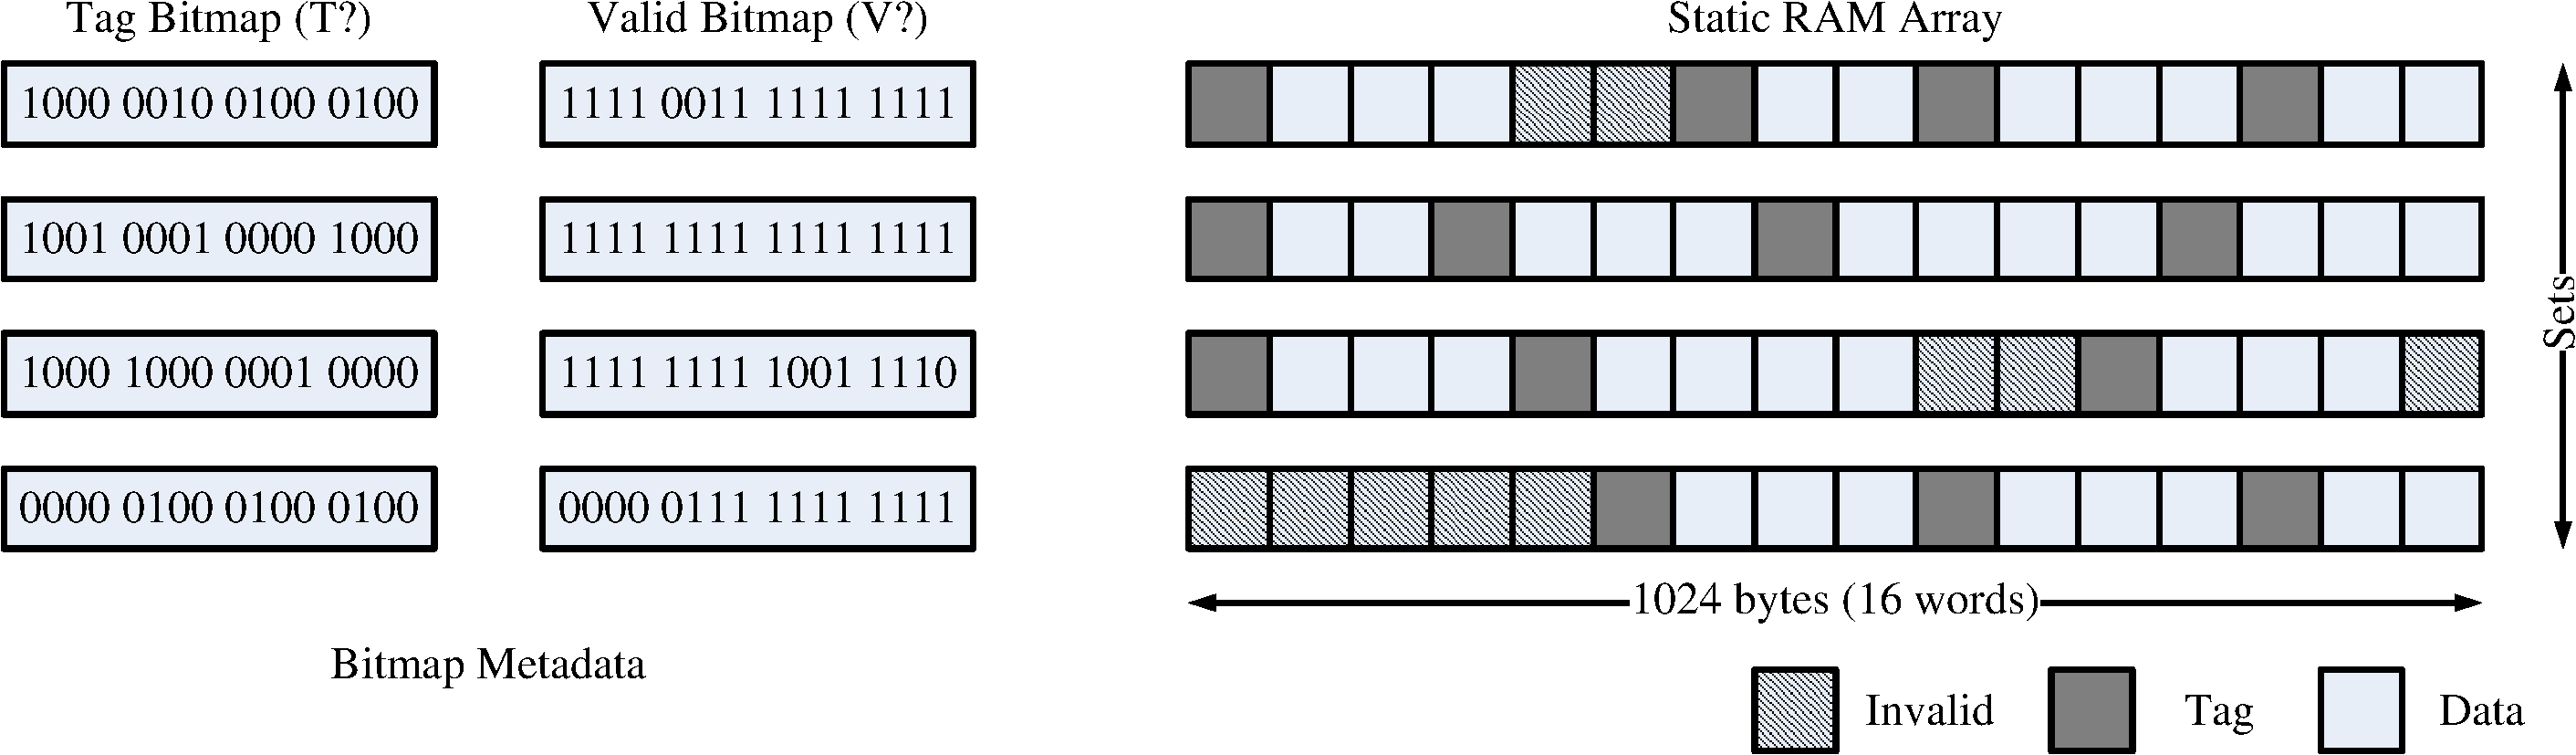
\includegraphics[width=\textwidth]{files/Figures/06-AmoebaCacheArch.pdf}
    \caption[Amoeba Cache Overview]{\textbf{Amoeba Cache Overview} The static RAM (SRAM) array where the tags and data are colocated is shown on the right. The \code{T? Bitmap} and the \code{V? Bitmap} for the \AC\ are shown on the left. Each block in the SRAM array represents 8 bytes (1 word). In this specific example, we show an \AC\ with 4 sets and 1024 bytes per set. The invalid, data and tag words (marked in the SRAM array) are tracked by setting the corresponding bits in the \code{T? and V? Bitmaps}. This information is maintained in order to simplify cache operations such as insertion and refill. }
    \label{fig:amoeba_cache_arch}
  \end{center}
\end{figure}

The \AC\ adopts a solution inspired by software data structures, where programs hold meta-data and actual data entries in the same address space. To achieve maximum flexibility, the \AC\ completely eliminates the tag array and collocates the tags with the actual data blocks (see Figure~\ref{fig:amoeba_cache_arch}). To distinguish which words are data words and which ones are tags within the set, we use a bitmap data structure (labeled \code{T? Bitmap} in Fig~\ref{fig:amoeba_cache_arch}). For each word in the set which is a tag, we set the corresponding bit in the \code{T? Bitmap}. We also decouple the conventional valid/invalid bits (typically associated with the tags) and organize them into a separate array (labeled \code{V? Bitmap} in Fig~\ref{fig:amoeba_cache_arch}) to simplify block replacement and insertion. \AC\ tags are composed of a \code{Region Tag} and a tuple which consists of the \code{Start} and \code{End} address of the variable granularity cache block. The data block immediately follows the tag word as shown in Fig~\ref{fig:amoeba_cache_arch}. The following sections provide more detail about the \AC\ architecture and how cache operations are performed.


\section{Amoeba Blocks and Set-Indexing}
\label{sec:amoeba_blocks_and_set_indexing}

\begin{figure}[h]
  %% Get images from http://en.wikipedia.org/wiki/CPU_cache#Associativity
  \subfloat[Memory Regions]{
    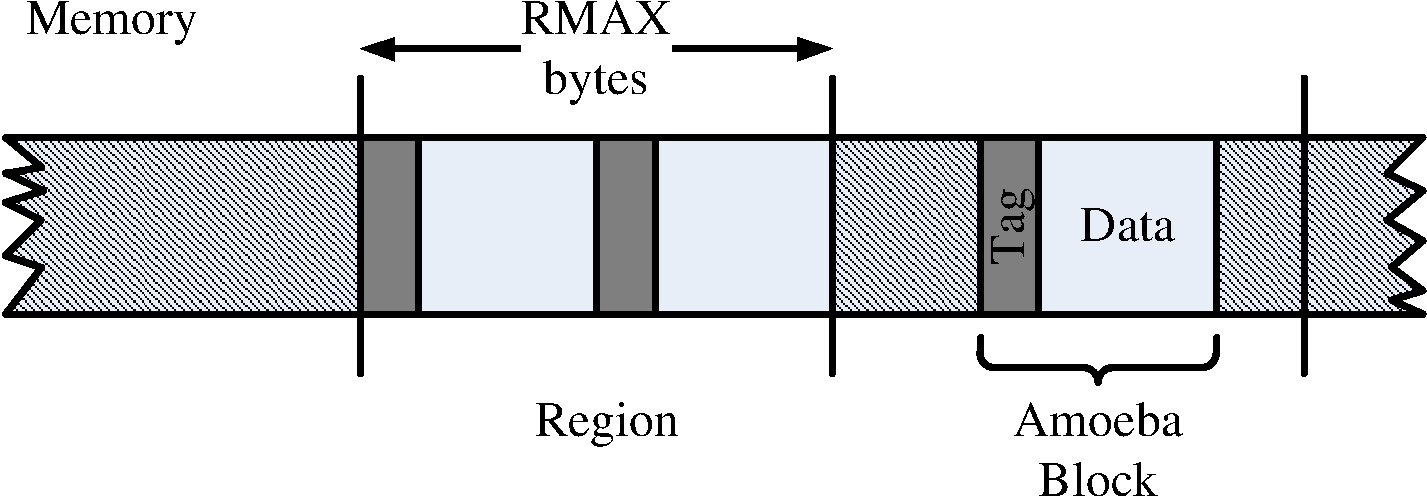
\includegraphics[width=0.5\textwidth]{files/Figures/06-MemoryRegions.pdf}
  }
  \subfloat[Addressing]{
     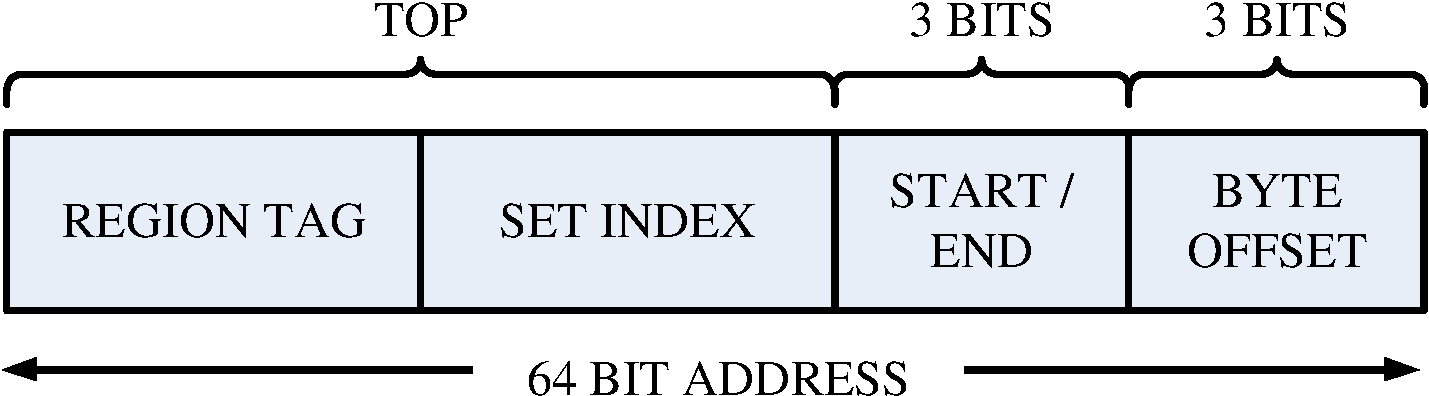
\includegraphics[width=0.5\textwidth]{files/Figures/06-Addressing.pdf}
  }
  \caption[Memory Regions]{ (a) The linear memory address space is segmented into Regions. The \AB{}s are constrainted to have their start and end within a single memory region. (b) 64 bits are used to encode the Region Tag, the Set Index, the start or end word and the word offset in the tag for an \AB{}.  }
  \label{fig:mem_region_addr}
\end{figure}


The \AC\ data array holds a collection of varied granularity \AB{}s that do not overlap. Each \AB\ is a 4 tuple consisting of \code{\textless RegionTag, Start, End, Data-Block\textgreater} (Figure~\ref{fig:amoeba_cache_arch}). The first 3 components of the tuple are equivalent to a tag in a conventional cache. We allocate 8 bytes (1 word) for each tag. In order to simplify cache lookups for \AB{}s, we partition the address space into \code{Regions}. A \code{Region} is an aligned block of memory of size \code{RMAX} bytes. The boundaries of any \AB{} block (\code{Start} and \code{End}) are constrained to lie within the regions' boundaries. The minimum granularity of the data in an \AB\ is 1 word and the maximum is \code{RMAX} words. We can encode \code{Start} and \code{End} in $log_2(RMAX)$ bits. The set indexing function masks the lower $log_2(RMAX)$ bits to ensure that all \AB{}s (every memory word) from a region index to the same set. The Region Tag and Set-Index are identical for every word in the \AB{}. Retaining the notion of \textit{sets} enables fast lookups and helps elude challenges such as synonyms (same memory word mapping to different sets). When comparing against a conventional cache, we set \code{RMAX} to 8 words (64 bytes), ensuring that the set indexing function is identical to that in the conventional cache to allow for a fair evaluation.



\section{Data Lookup}

When data is referenced by the CPU, a cache lookup takes place in order to determine whether the required datum is present in the cache or not (resulting in a cache hit or miss). The operation percolates down the memory hierarchy until a cache returns a hit or the backing store supplies the datum required. Fig~\ref{fig:set_assoc_arch} shows a conventional cache which operates in \textit{Fast Mode}, where the contents of the entire set is read out into the output buffer in parallel with the tag lookup. Megabyte sized caches, with larger sets, may want to avoid the extra cost of reading out all ways to the output buffer and wait until the tag lookup completes to read out only the correct way from the set. Though this saves energy, it serializes the lookup and takes longer. The delay is usually tolerated as the \textit{Serial Mode} lookup is often implemented in the L2 caches or lower in the memory heirarchy. Another approach which minimises energy whilst still reading out the way in parallel is \textit{way prediction}\cite{patent:DataCacheWayPrediction,patent:WayPredictionVirtualHint}, commonly used in processors manufactured by MIPS.
\\

In contrast to a conventional cache, the \AC\ needs to lookup tags from the SRAM array to determine a hit or miss. The metadata stored in the \code{T? Bitmap} is used during the lookup operation in the \AC{}. Figure~\ref{fig:ac_lookup} describes the steps of the lookup procedure in an \AC{}. The overheads incurred due to the extra stages introduced in the critical path are evaluated in chapter \ref{sec:hardware_complexity}.


\begin{figure}[h]
  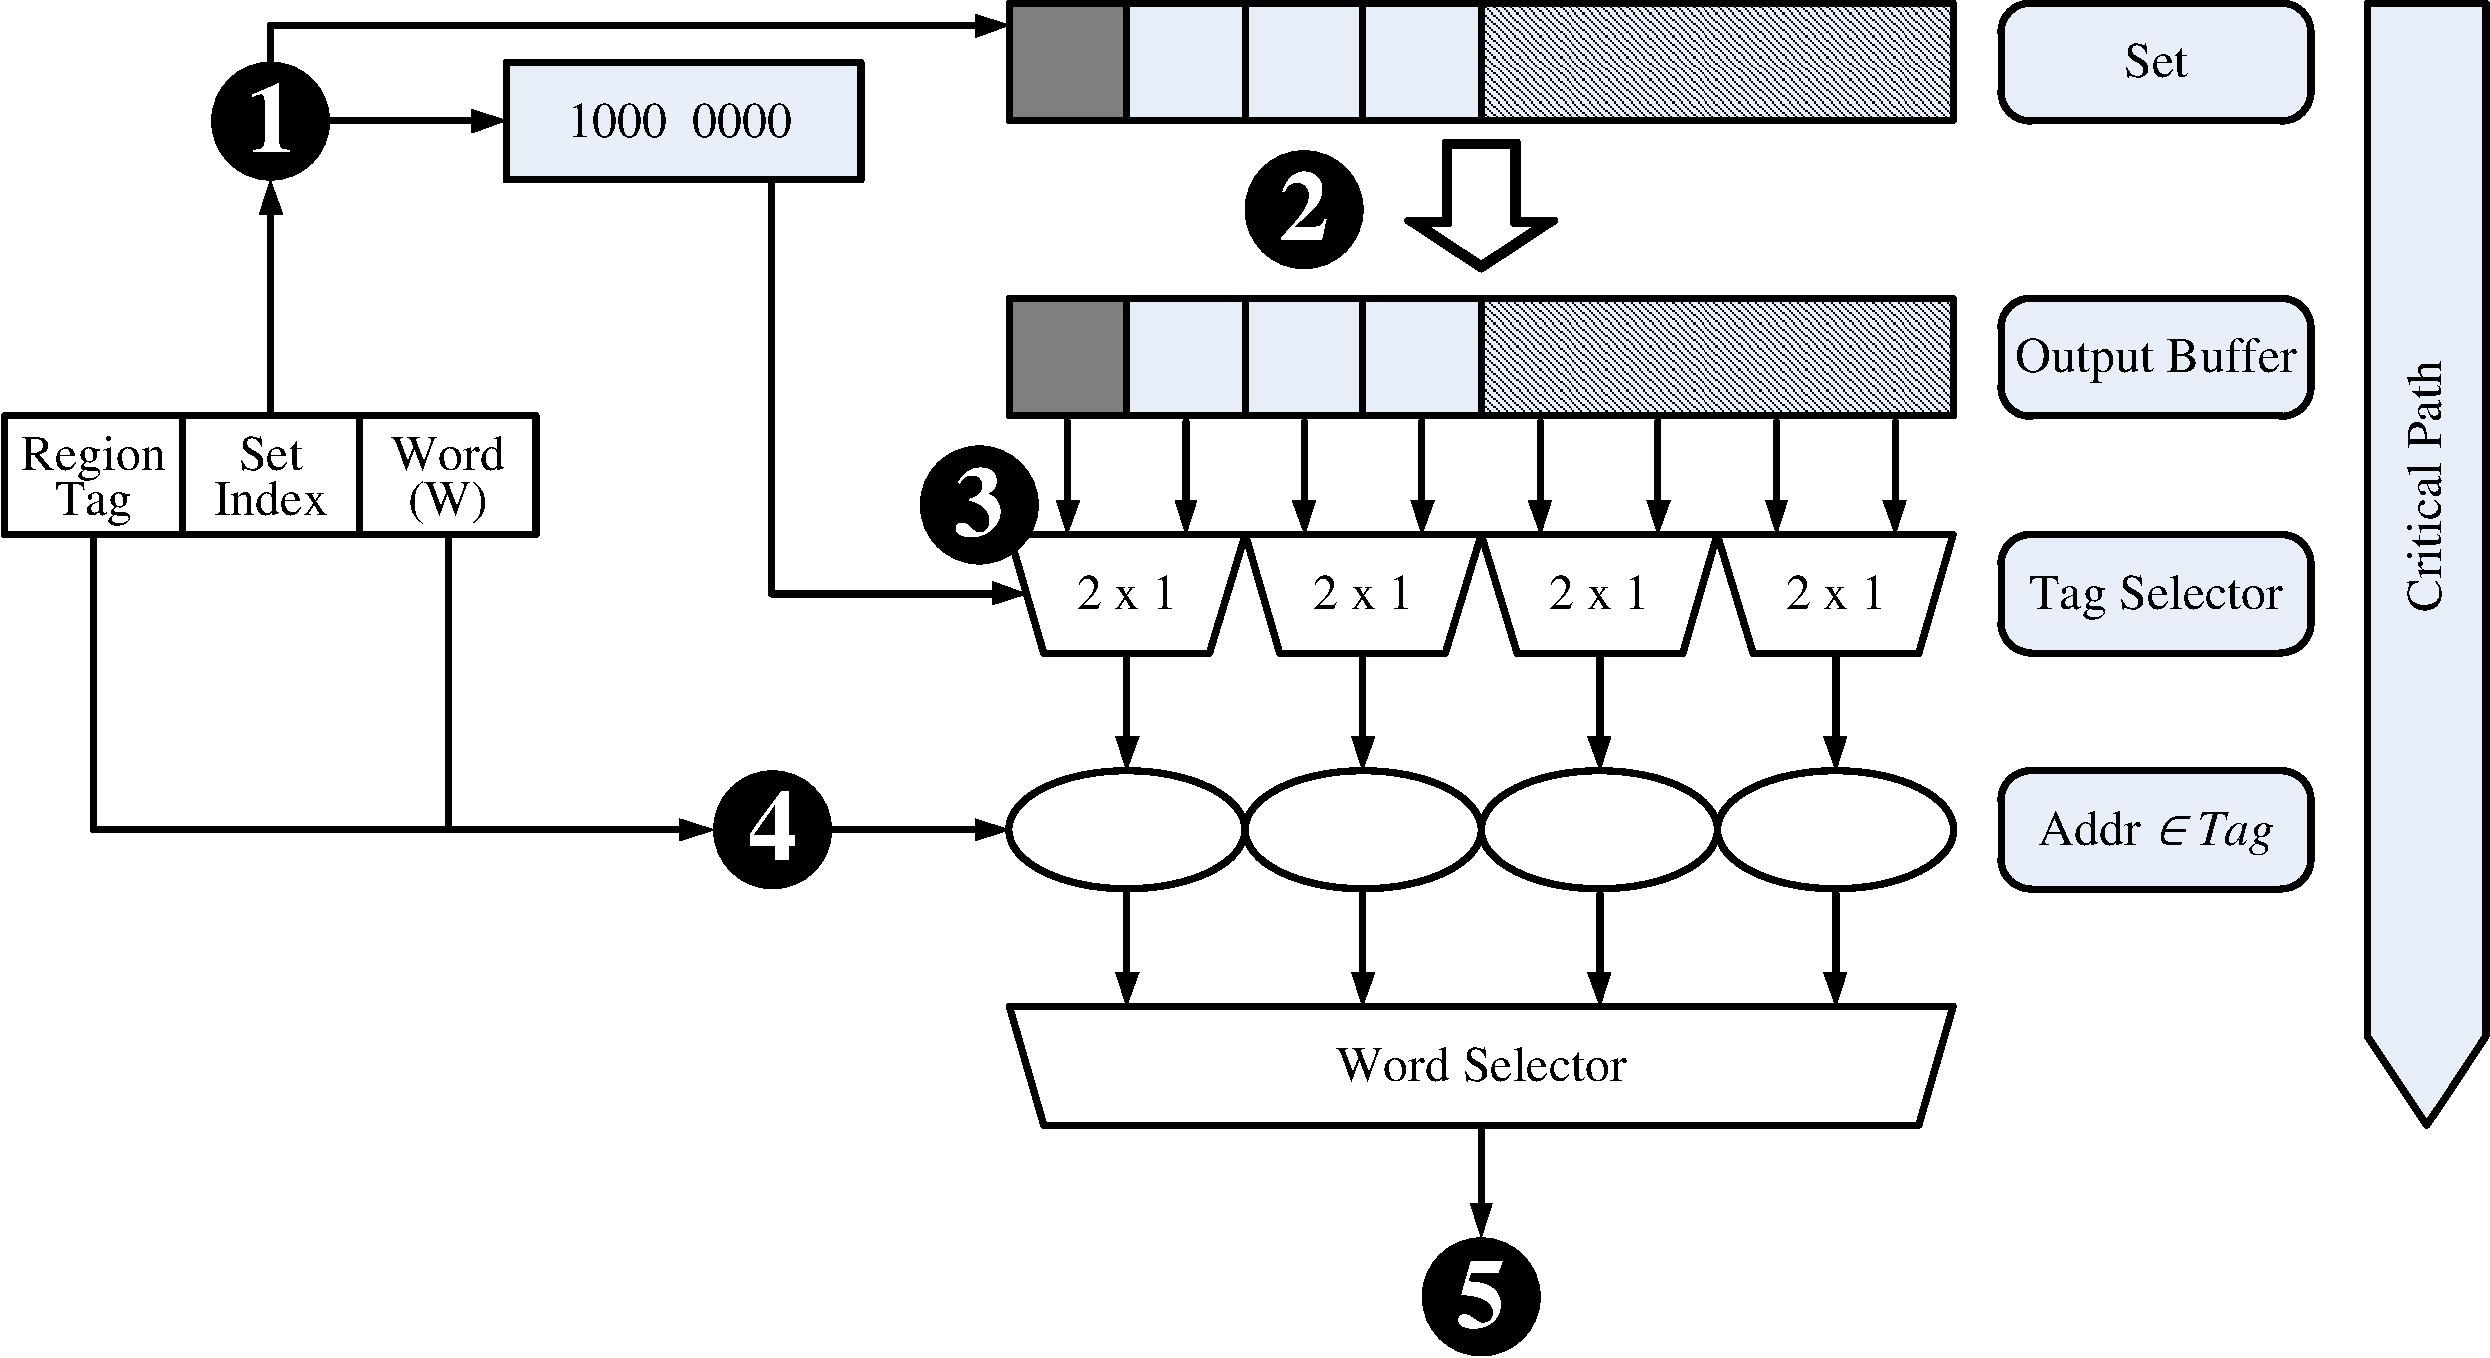
\includegraphics[width=\textwidth]{files/Figures/06-Lookup.pdf}
  \caption[Amoeba Cache Lookup]{\textbf{Amoeba Cache Lookup} : The incoming effective address is segmented into the region tag, set index and word offset. \bigspot{1} The \code{Tag? Bitmap} is looked up to determine which words in the activated set are required for the tag comparison. Note that given the minimum size of a \AB{} is two words (1 word for the tag metadata, 1 word for the data), adjacent words cannot be tags. Given this constraint, 
  the number of 2-1 multiplexers required to route one of the adjacent words to the comparator ($\in$ operator), is equal to half the number of words in the set. \bigspot{2} Simultaneously, the set is activated and the contents are latched onto the output buffer. \bigspot{3} The appropriate tag words are selected with the input from the the \code{Tag? Bitmap}. \bigspot{4} The comparator generates the hit signal for the word selector. The $\in$ operator consists of two comparators: a) an aligned \code{Region tag} comparator, a conventional $==$ (64 - $log_2N_{sets}$ - $log_2{RMAX}$ bits wide, e.g., 50 bits) that checks if the \AB{} belongs to the same region and b) a $ Start <= W < END $ range comparator ($log_2RMAX$ bits wide; e.g., 3 bits) that checks if the \AB\ holds the required word. Finally, in \bigspot{5}, the tag match activates and selects the appropriate word. The critical path (as indicated on the left) includes the read out from the set, the tag selectors and the $\in$ operation.}
  \label{fig:ac_lookup}
\end{figure}

\clearpage

\section{Block Insertion}

On a miss for the desired word, a spatial granularity predictor is invoked (see Section~\ref{sec:spatial_pattern_predictor}), which specifies the range of the \AB{} to refill. To determine a position in the set to slot the incoming block we can leverage the \code{Valid? Bitmap}. The \code{V? Bitmap} has 1 bit/word in the cache; a ``1'' bit indicates the word has been allocated (valid data or a tag). To find space for an incoming data block we perform a substring search on the \code{V? Bitmap} of the cache set for contiguous 0s (empty words). For example, to insert an \AB{} of five words (four words for data and one word for tag), we perform a substring search for \textit{00000} in the \code{V? Bitmap} / set (e.g., 32 bits wide for a 64K cache). If we cannot find the space, we keep triggering the replacement algorithm until we create the requisite contiguous space. Following this, the \AB\ tuple (Tag and Data block) is inserted, and the corresponding bits in the \code{T? and V? Bitmaps} are set. The 0s substring search can be accomplished with a lookup table; many current processors already include a substring instruction. Intel SSE 4.2 include the instruction, \code{PCMPISTRI}, which can accomplish the required task.

\section{Replacement Policy}

The replacement policy of a cache determines which blocks are evicted when new data is brought in and there is no room to store it. The replacement algorithm tries to make an optimal choice where it evicts a blocks which is not expected to be used in the near future. The most optimal choice possible would be to remove a block which is not going to be referenced in the program again or which is going to be referenced farthest in the future in comparison to the other cache blocks. The optimal algorithm is also known as \textit{"Belady's Optimal Algorithm"}, named after Hungarian computer scientist, Laszlo Belady.
\\

The Least Recently Used (LRU) algorithm is a popular choice for conventional caches and is based on the principle of temporal locality of reference. The hardware tracks data reference to the different cache blocks and when a new insertion request arrives, the least recently used block in the set is evicted. Implementing an LRU cache in software is relatively easy with the use of a linked list. Hardware manufacturers commonly implement the \textit{Pseudo-LRU}(PLRU) which has a lower metadata overhead and is a reasonable approximation of LRU. The tree based PLRU was implemented in processors such as the Intel 80486 and many processors in the PowerPC family. 

\subsection{Pseudo-LRU}

The tree based Pseudo-LRU algorithm was developed as an approximation of LRU due to the exponentially increasing complexity of storing the LRU state for increasing number of ways (an $N_{way}$ cache would require $N!$ states). For multi threaded processor designs and megabyte sized caches, it is often desirable to have a high level of associativity. For Pseudo-LRU, one bit indicates whether the most recent reference is to a line in either the first half or the second half of the lines in a set; then, this technique is logically applied recursively, resulting in a logical binary tree with N-1 nodes (thus N-1 bits are required to represent a state in tree-PLRU). A 4-way set associative can be encoded for PLRU replacement with 3 bits. Each bit represents one branch point in a binary decision tree; let 1 represent that the left side has been referenced more recently than the right side, and 0 vice-versa. 
\\ 
\begin{figure}[hb]
  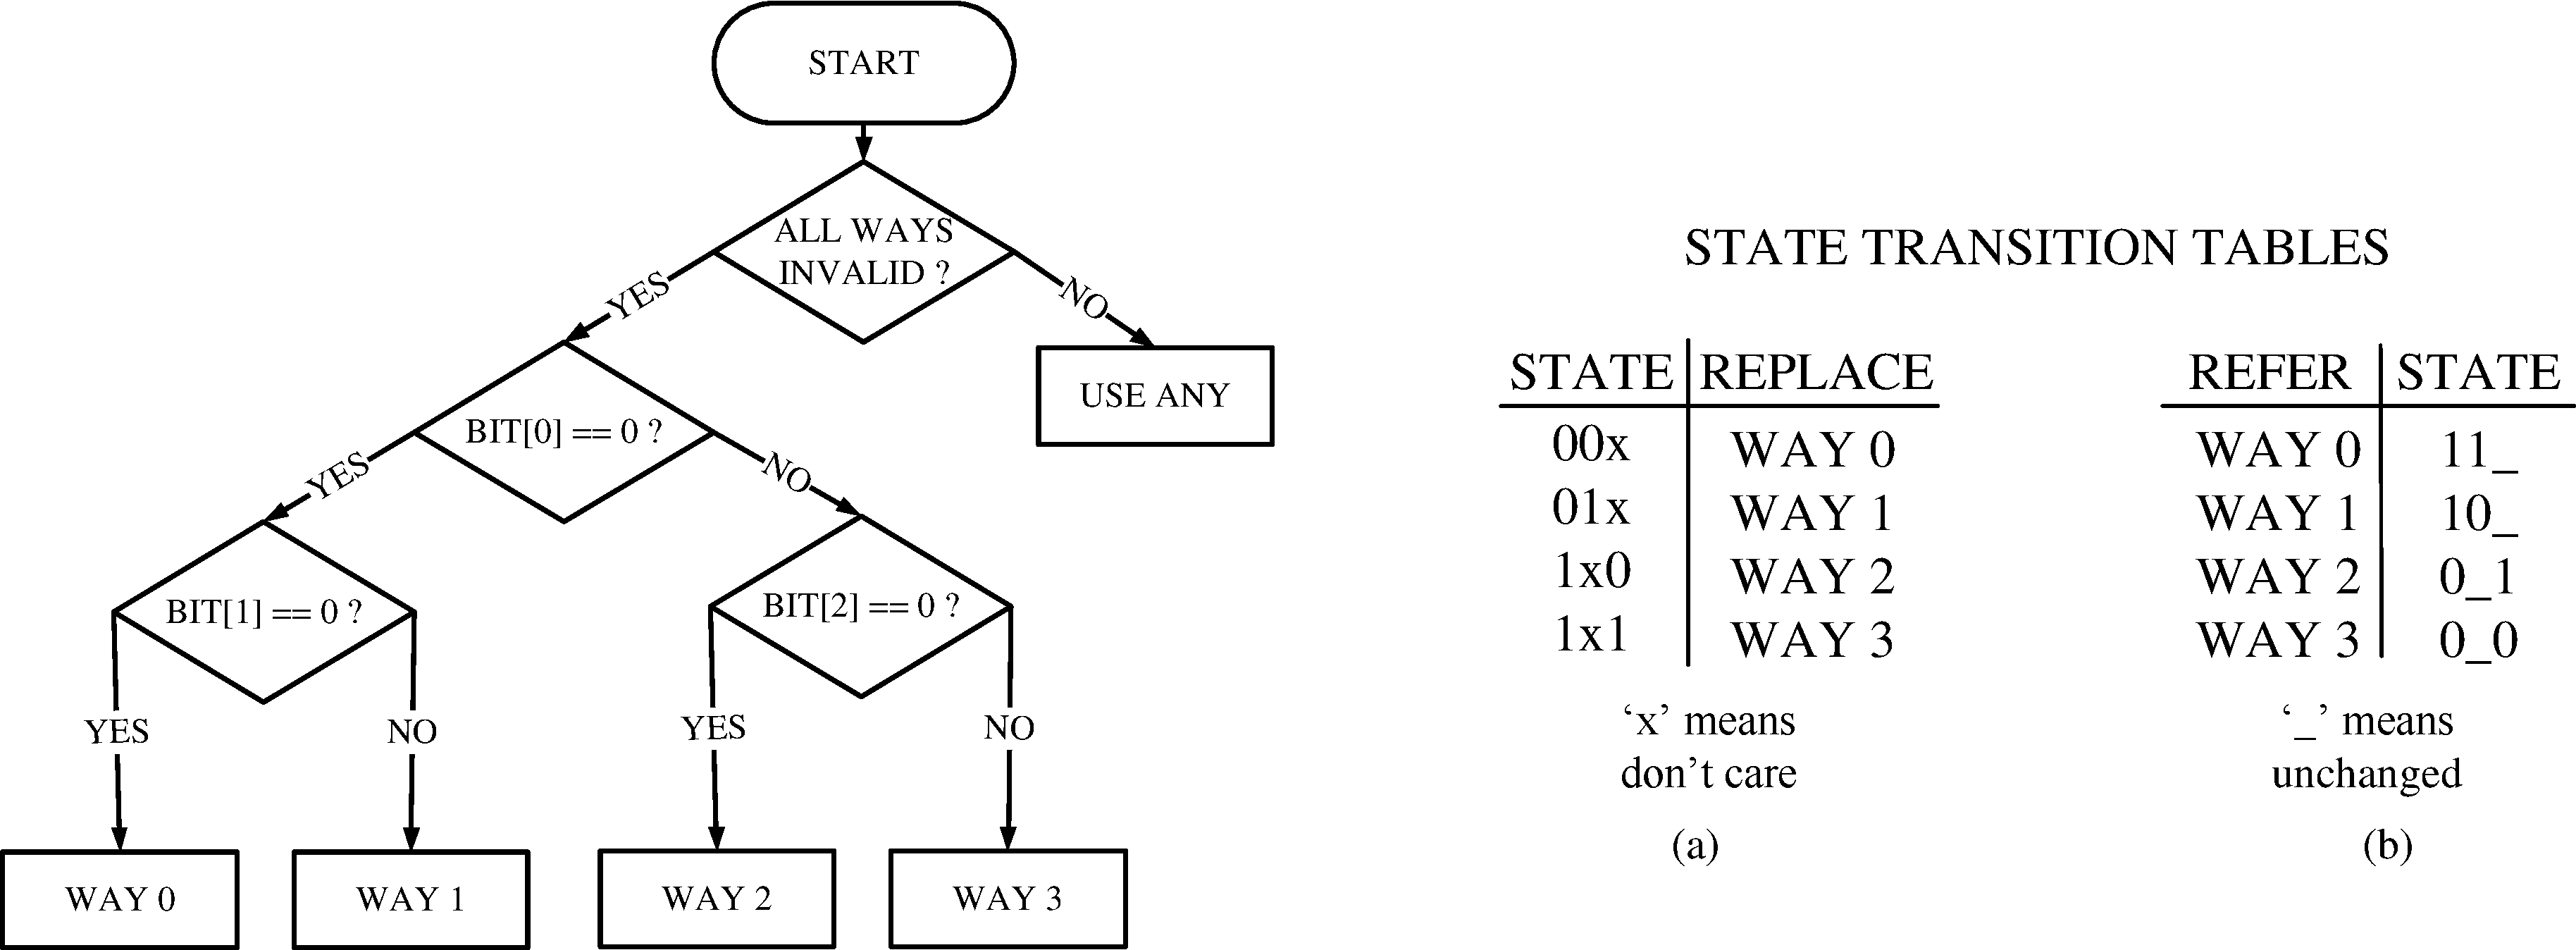
\includegraphics[width=\textwidth]{files/Figures/06-PLRU.pdf}
  \\
  \caption[Pseudo LRU]{\textbf{Pseudo-LRU decision tree and state transition table} : The flowchart on the left shows the decision making process based on the values of the 3 PLRU bits in a 4-way associative cache. The state transition tables on the right are (a) way to replace for given state (b) state to transition to on reference to a way. Reproduced from Intel Embedded Pentium Processor Family Dev. Manual\cite{manual:IntelProcessor}.}
  \label{fig:plru}
\end{figure}

\subsection{\AC\ Replacement Policy}

To reclaim the space from an \AB\, the tag bits T? (tag) and V? (valid) bits corresponding to the block are unset. The key issue is identifying the \AB\ to replace. Classical pseudo-LRU algorithms~\cite{Kedzierski-ipdps-2010,manual:OpenSparcT1} keep the metadata for the replacement algorithm separate from the tags to reduce port contention. To be compatible with pseudo-LRU and other algorithms such as DIP~\cite{qureshi-isca-2007} that work with a fixed number of ways, we can logically partition a set in \AC\ into $N_{ways}$. For instance, if we partition a 32 word cache set into 4 logical ways, any access to an \AB\ tag found in words 0 ---7 of the set is treated as an access to logical way 0. Finding a replacement candidate involves identifying the selected replacement way and then picking (possibly randomly) a candidate \AB{}. This procedure is repeated until the required amount of space is made available. More refined replacement algorithms that require per-tag metadata can harvest the space in the tag-word of the \AB\, which is 64 bits wide (for alignment purposes) while physical addresses rarely extend beyond 48 bits.

\section{Partial Misses} 
\label{sec:partialmiss} 

With variable granularity data blocks, a challenging although rare case (5 in every 1K accesses) that occurs is a \textit{partial miss}. It is observed primarily when the spatial locality changes.  Figure~\ref{fig:partial-miss} shows an example. Initially, the set contains two blocks from the region R, one \AB\ caches words 0 --- 2 (Region:R Start:0 End:2) and the other caches words 6 and 7 (Region:R Start:6 End:7). Let us assume that the CPU reads word 4, which misses, and the spatial pattern predictor requests an \AB\ with range Start:0 and End:7. The cache has \AB{}s that hold subparts of the incoming \AB{}, and only some words (4,5 and 5) need to be fetched.

\begin{figure}[h]
  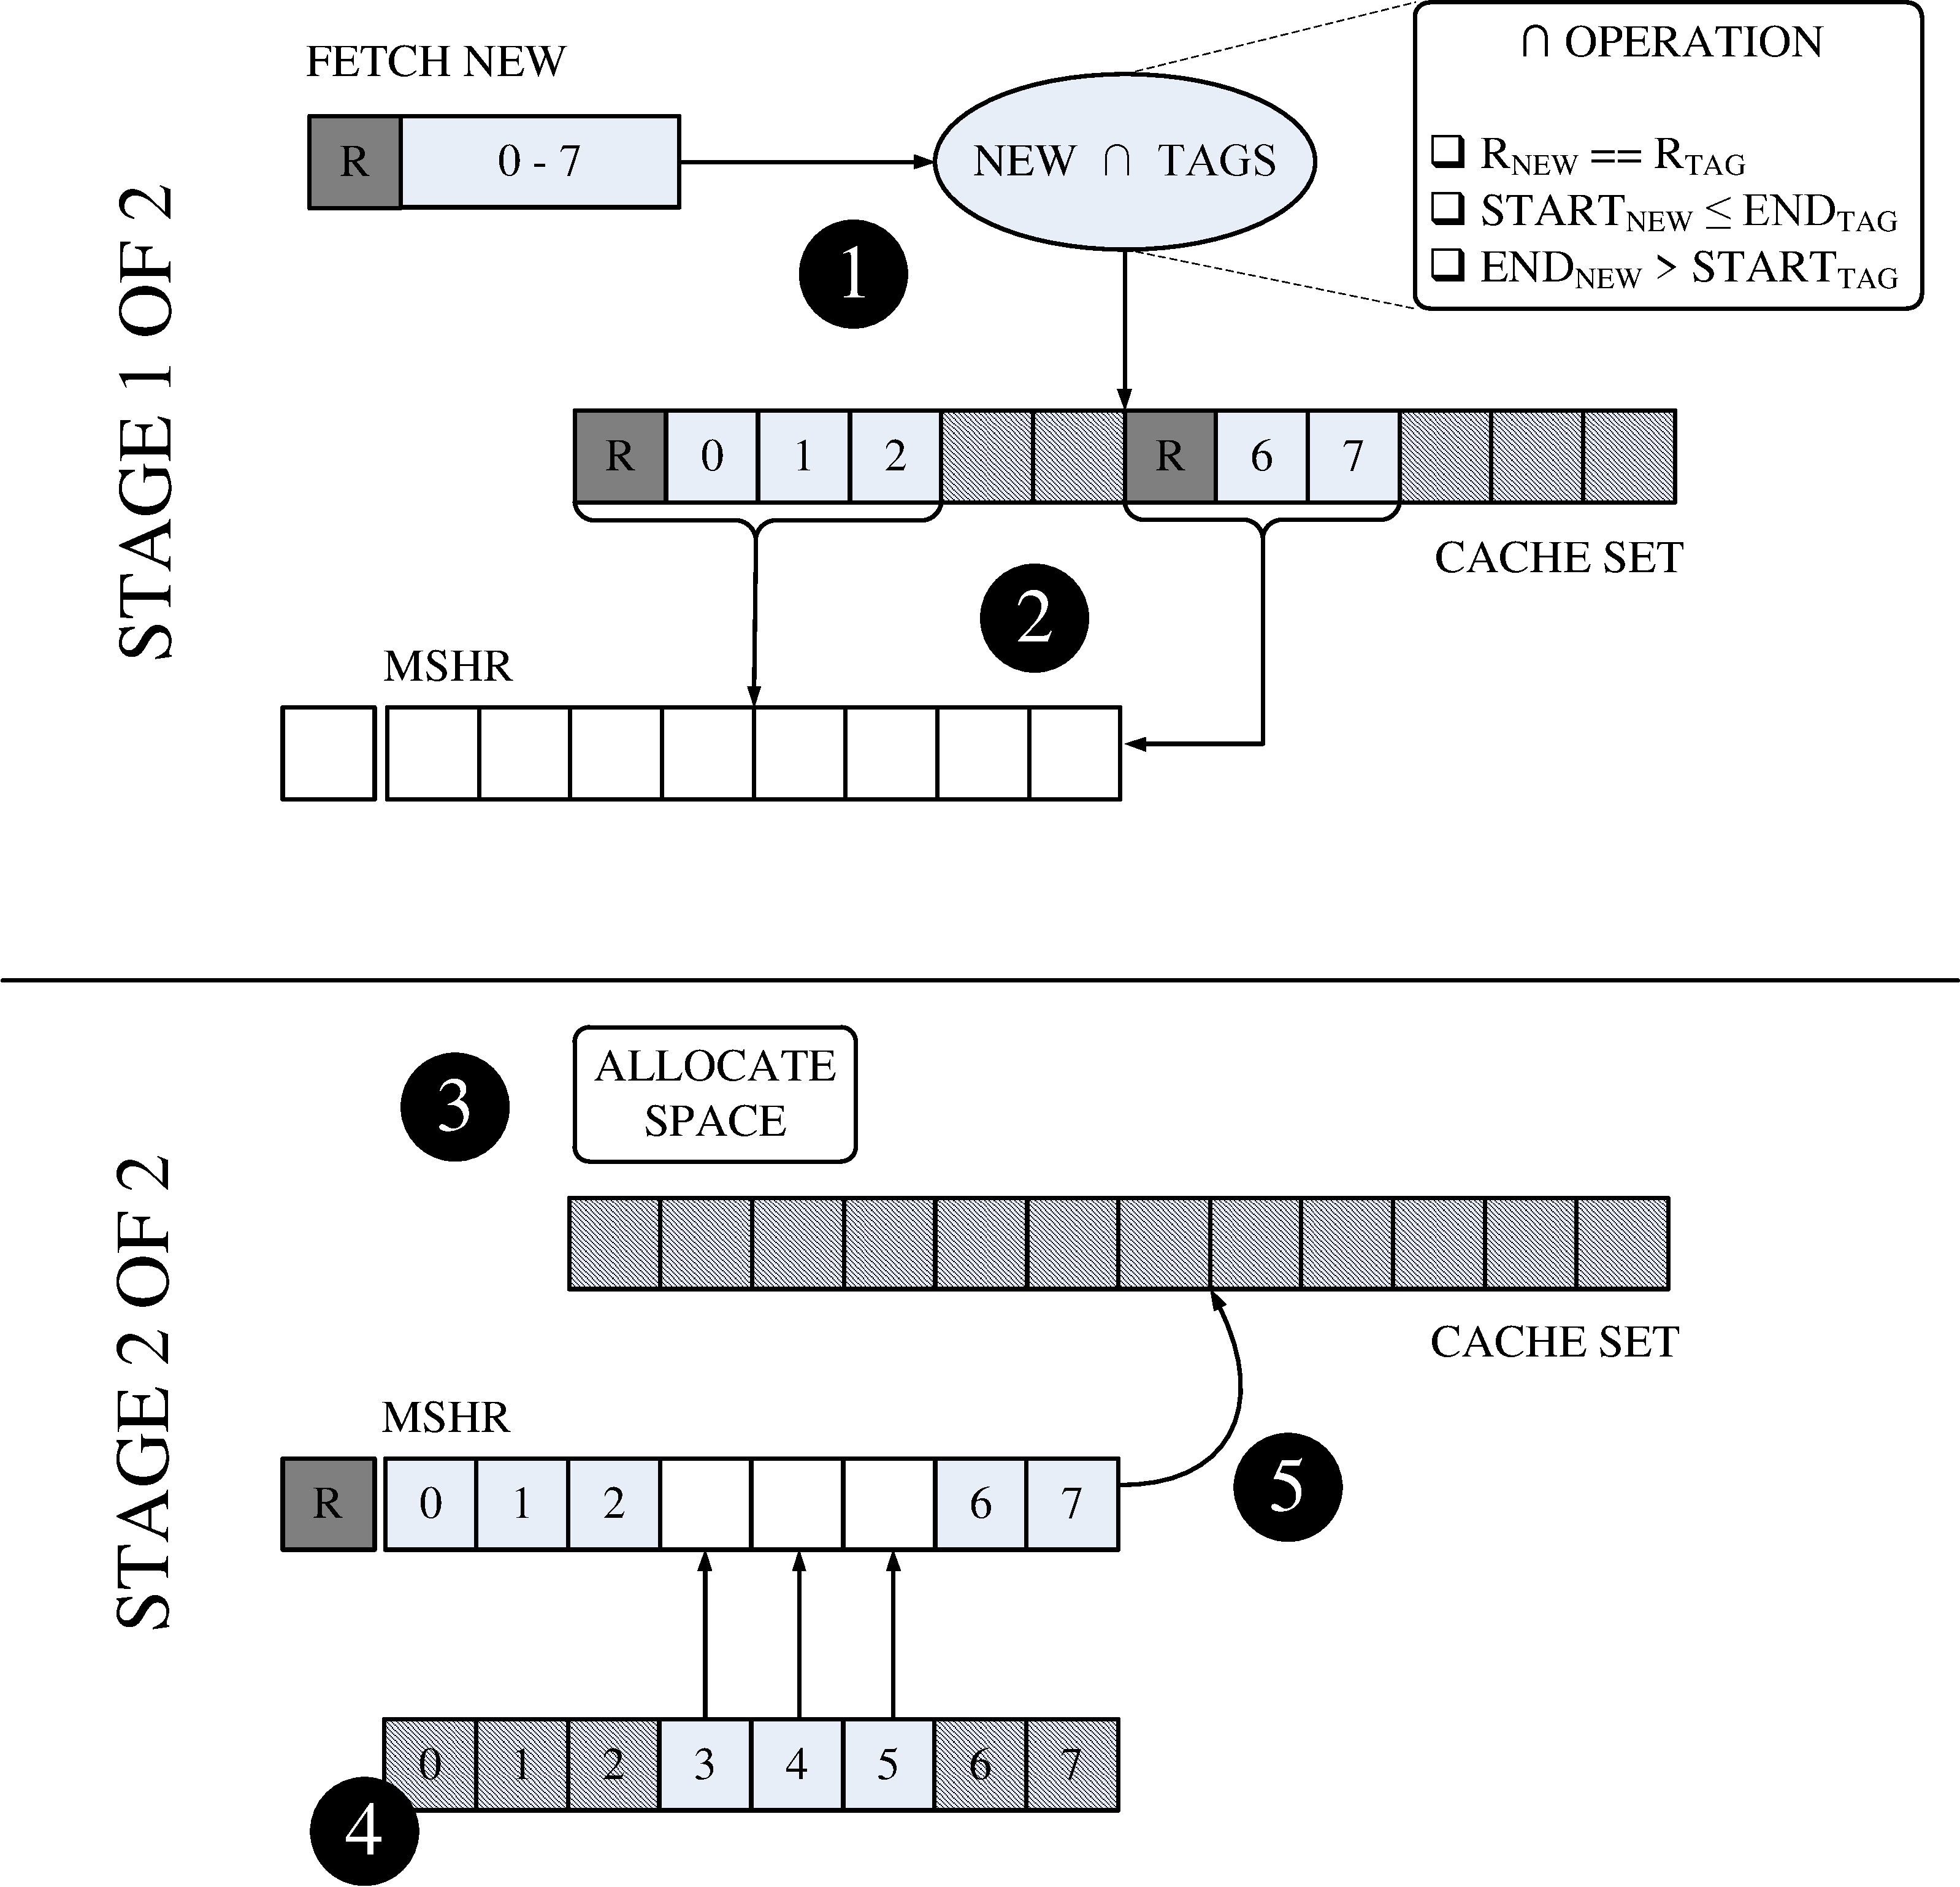
\includegraphics[width=\textwidth]{files/Figures/06-PartialMiss.pdf}
  \\
  \caption[Partial Miss]{\textbf{Partial miss processing} : The partial miss processing is shown as 2 separate stages. Stage 1 deals with the identification and eviction (to MSHR) of all overlapping blocks. Stage 2 issues the miss, allocates space for the new \AB\ and patches in the missing words from a lower level in the memory hierarchy before copying the data back into the cache set. Due to the infrequent nature of partial misses we do not optimise for fetching only the missing words in our implementation. }
  \label{fig:partial-miss}
\end{figure}

\clearpage

\AC\ removes the overlapping sub-blocks and allocates a new \AB{}. This is a multiple step process: \bigspot{1} On a miss, the cache identifies the overlapping sub-blocks in the cache using the tags read out during lookup. The $\cap$(in) operation returns false if there are no overlapping blocks. The $\cap$ operation consists of an equality check for the region (R), $Start_{New} \leq End_{Tag}$ and $End_{New} > Start_{Tag}$ (where \textit{New} refers to the fetch request from the spatial pattern predictor and \textit{Tag} refers to the existing \AB{}). \bigspot{2} The data blocks that overlap with the miss range are evicted and moved one-at-a-time to the miss status holding register (MSHR) entry. \bigspot{3} Space is then allocated for the new block, i.e., it is treated like a new insertion. A miss request is issued for the entire block (Start:0 --- End:7) even if only some words (e.g., 3, 4 and 5) may be needed. This ensures request processing is simple and only a single refill request is sent. \bigspot{4} The incoming data block is patched into the MSHR; only the words not obtained from the L1 (words 3,4 and 5 as indicated in Fig\ref{fig:partial-miss}) are copied (since the lower level could be stale). \bigspot{5} The entire block is copied back into the SRAM array.

\section{Spatial Pattern Predictor}
\label{sec:spatial_pattern_predictor}

The \AC\ uses a spatial block predictor, which  informs refill requests about the range of the block to fetch. \AC\ can exploit any spatial locality predictor and there have been many efforts in the compiler and architecture community~\cite{Chilimbi-Hill-pldi-1999, kumar-isca-1998, pujara-hpca-2006,chen-hpca-2004}. We adopt a tabular approach, as shown in Fig~\ref{fig:predictor}, consisting of a set of access bitmaps; each entry is \code{RMAX} (maximum granularity of an \AB{}) bits wide and represents whether the word was touched during the lifetime of the recently evicted cache block. The entry is indexed with information gleaned from either the program counter (PC) which initiated the cache miss or region tag for the effective address or both. On a miss, the predictor will search for an entry  and choose the range of words to be fetched on a miss on either side (left and right) of the critical word. The predictor optimizes for spatial prefetching and will  overfetch (bring in potentially untouched words), if they are interspersed amongst contiguous chunks of touched words. We can also bypass the prediction when there is low confidence in the prediction accuracy, i.e. when there may not be an entry in the table. We evaluate tradeoffs in the design of the spatial predictor in Section~\ref{sec:predictor_tradeoffs}.


\begin{figure}[h]
  \centering
  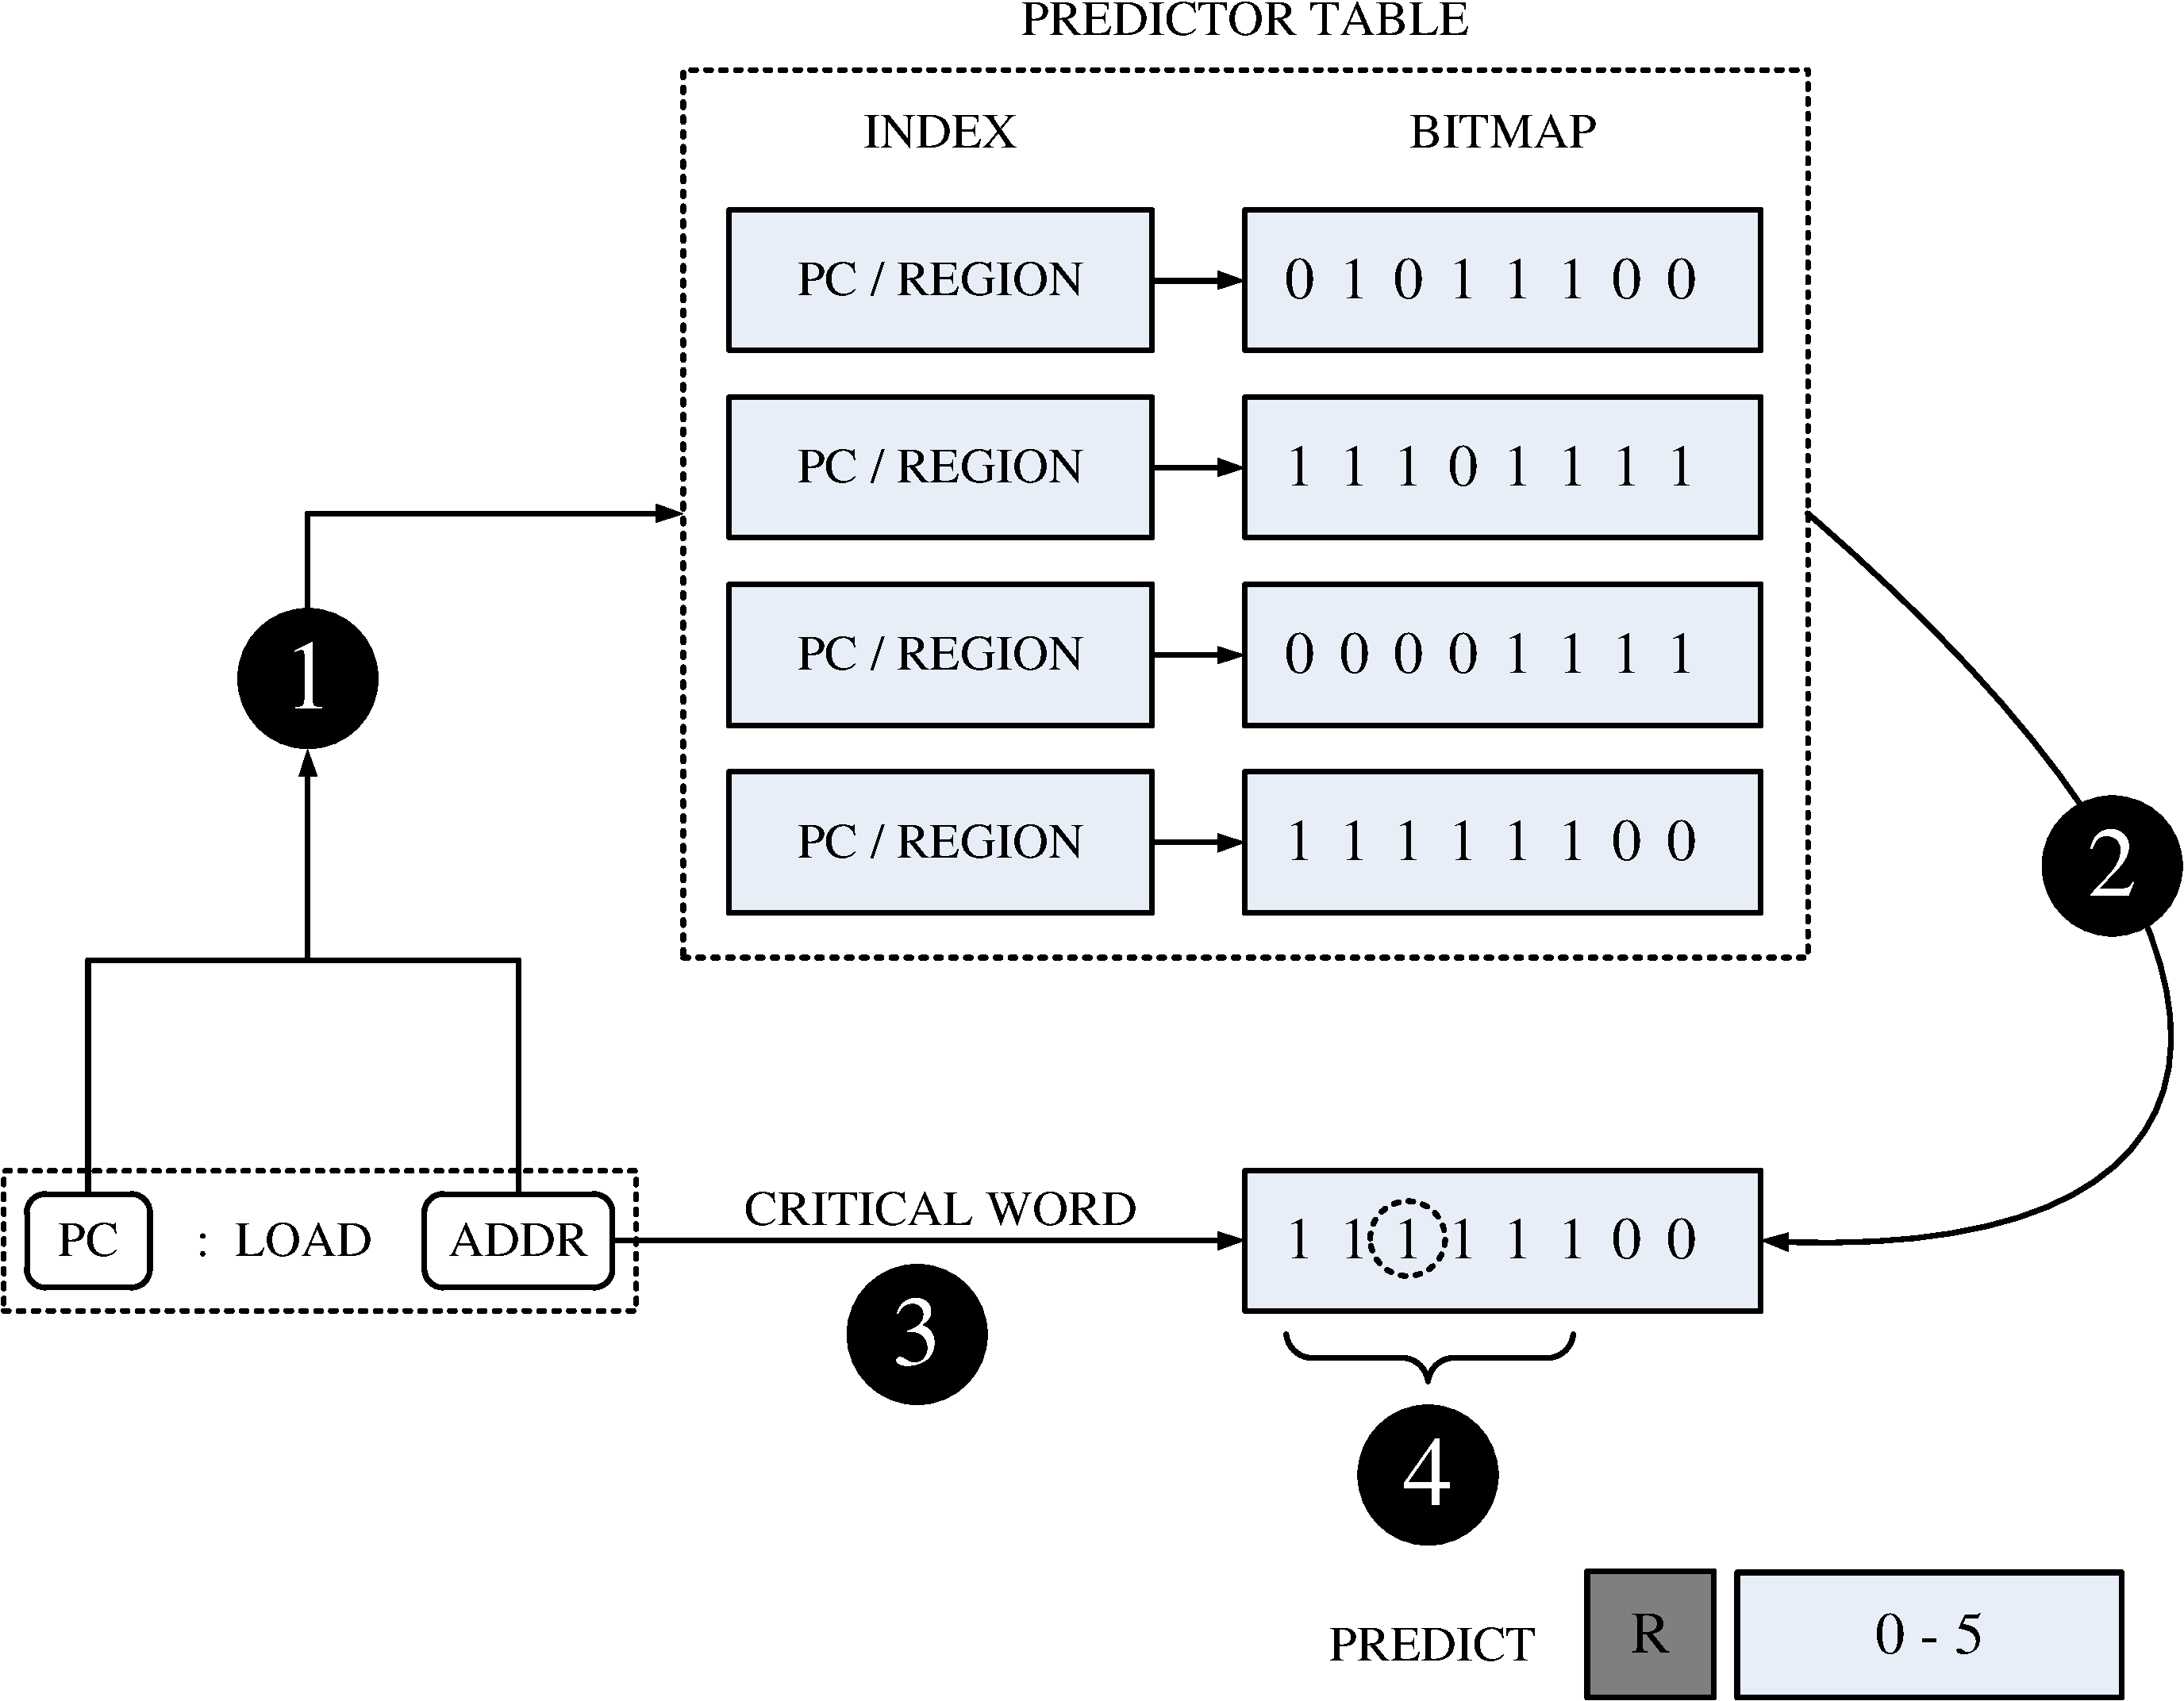
\includegraphics[width=0.75\textwidth]{files/Figures/06-Predictor.pdf}
  \\
  \caption[Amoeba-Cache Predictor]{\textbf{\AC\ Predictor} : On a cache miss, the \AC\ predictor performs the following steps. \bigspot{1} Lookup the table using bits from the program counter or region tag or a combination of both. \bigspot{2} If an entry is present for the calculated index, the corresponding bitmap is read out from the table. The bitmap is updated on eviction of a cache block with the pattern of words accessed by the CPU in the cache block during its lifetime. \bigspot{3} We examine the critical word (word requested by the instruction), to ensure it is part of the marked portion of the bitmap. We then extend the range for the new block to include all marked words in the bitmap. \bigspot{4} The predictor then requests the cache to issue a miss for words 0 -- 5 based on the bitmap pattern.}
  \label{fig:predictor}
\end{figure}

\section{Related Work}

In this section we look at prior work in the area which closely relate to the \AC{}. 

\subsection{Line Distillation}

\begin{figure}[h]
  \centering
  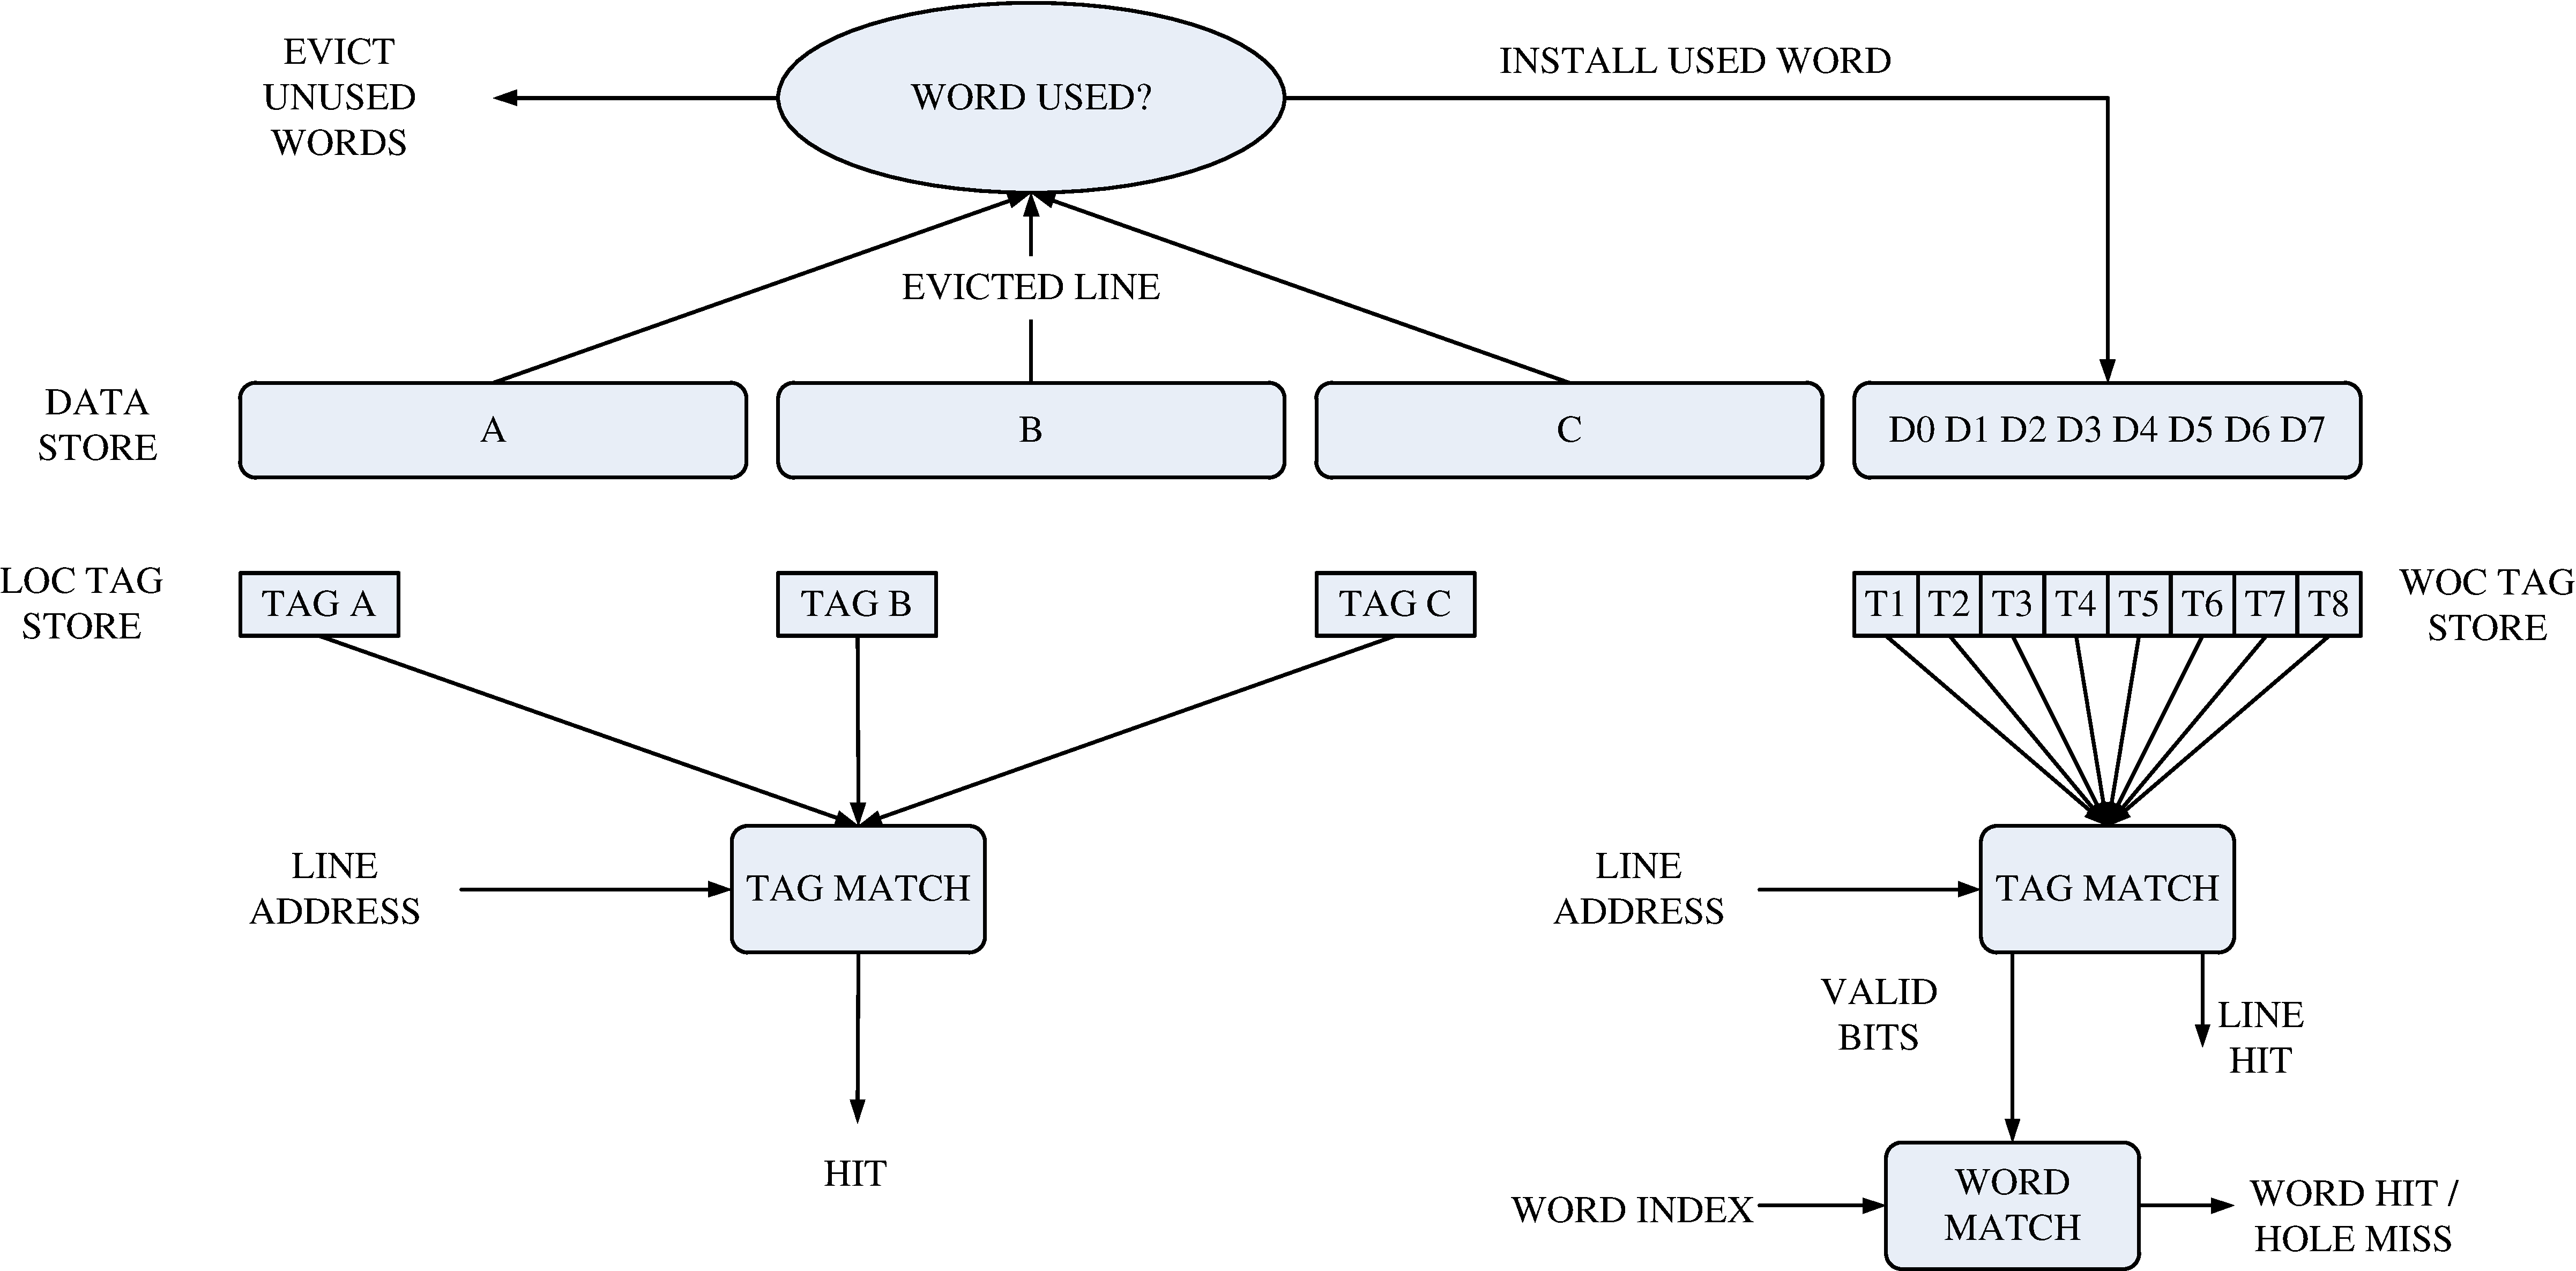
\includegraphics[width=\textwidth]{files/Figures/06-LDIS.pdf}
  \\
  \caption[Line Distillation]{\textbf{Line Distillation Organisation} : The figure shows a single set from a 4-way \textit{Distill Cache}. The LOC consists of ways A,B and C and the WOC consists of way D. A line evicted from the LOC ways is checked for suitable words to retain in the WOC. A lookup in the WOC includes a check for the line address as well as the word index to qualify as a hit.}
  \label{fig:ldis}
\end{figure}

Qureshi et al\cite{Qureshi:2007:LDIS} proposed a cache organisation dubbed as the \textit{Distill Cache} and a technique known as \textit{Line Distillation} to discard only the unused words from a cache line upon eviction. Their proposed organisation (as shown in Fig~\ref{fig:ldis}) includes a \textit{Line Organised Cache(LOC)} which stores blocks at the default line granularity (such as 64 bytes per line) and a \textit{Word Organised Cache(WOC)} which stores blocks at the granularity of a word (usually 8 bytes). The WOC is similar in spirit to the \textit{Victim Cache}\cite{Jouppi:1990:IDC:325164.325162} proposed by Jouppi. The victim cache is a small, fully associative cache which is usually coupled with a direct mapped cache and stores the victim of a cache miss. It was used to alleviate problems caused by conflict misses. The WOC however, does not cache the entire block. The WOC only caches the words within the cache block which were touched by the application at the time of eviction. Whether the words will be installed in the WOC or the entire line is discarded is determined by the number of words which were touched. The authors propose a \textit{median threshold filtering} policy, where the words are retained in the WOC on eviction only if the number of words touched in the cache line from the LOC is less than the median number of words touched in a cache block in the application. The authors propose the implementation of the \textit{Distill Cache} at the L2 as the design of the L1 data cache is is heavily constrained by cycle time and out of order processors already cover some of the latency of the cache misses. Their findings show an average improvement of 12\% in IPC by reducing cache misses for a 1MB 8-way L2 by 30\%.

The \textit{Distill Cache} is similar to the \AC\ in the sense that in a single cache it supports word granularity blocks and line granularity blocks as two extremes. The \AC\ supports varying granularity blocks of sizes 1--\textit{RMAX} words (see Section~\ref{sec:amoeba_blocks_and_set_indexing}). The WOC always incurs a high overhead in terms of a single tag for each of the data words in the WOC which is similar to the worst case scenario for an \AC\ where all the data words in the cache set are of size 1 word. Veidenbaum et al\cite{Veidenbaum:1999:ACL:305138.305188}, propose the entire cache be word organised and propose an online algorithm to prefetch required words. This approach however has a built in tag overhead of 50\% and requires energy intensive associative searches.

\subsection{Sector Caches}

The original cache designs\cite{liptay68} were essentially sector caches in nature was due to the technology available at the time (the discrete transistor logic for sectors was easier to implement) where the cache consisted of sectors (address tags) and subsectors (or blocks with valid bits). They were deprecated in favor of set associative caches which have superior performance in terms of miss rate and because many subsectors went unused due to early eviction of a sector (for a 64K data cache with 256 byte sector frame and 64 byte sector size had only 74\% utilization\cite{Rothman_Smith_2000}).
\\
\begin{figure}[h]
  \centering
  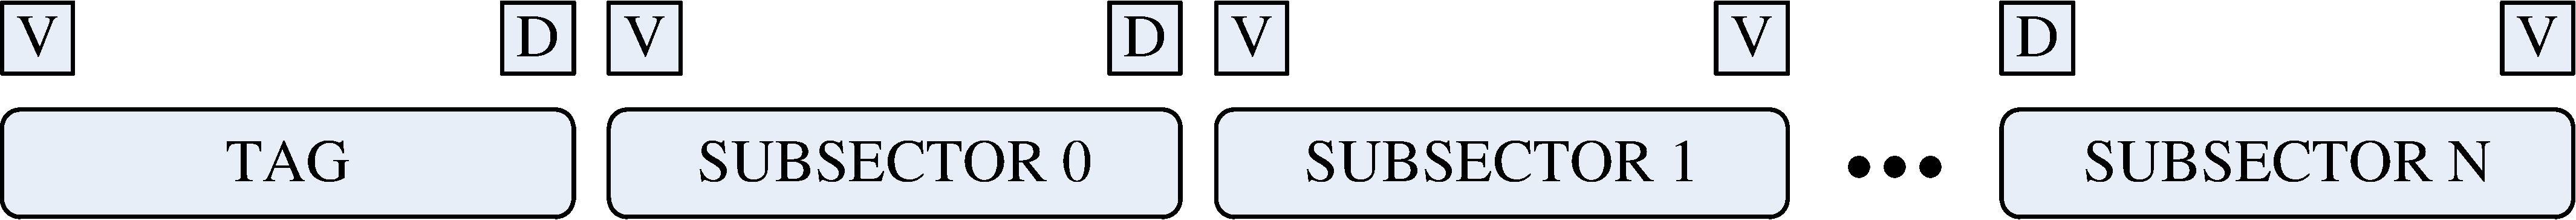
\includegraphics[width=\textwidth]{files/Figures/06-Sector.pdf}
  \\
  \caption[Sector Frame]{\textbf{Sector Frame} : Diagram of a single sector frame (reproduced from \cite{Rothman_Smith_2000}). \textit{D} is the dirty bit  and \textit{V} is the valid bit associated with the subsector. The first documented use of a cache in a computing system, the IBM 360/85, was 16 KBytes in size and consisted of 16 sector frames of 16 subsectors, each of size 64 byte blocks.}
  \label{fig:sector_frame}
\end{figure}

In the 90's interest in sector cache design was revived by Rothman et al\cite{Rothman_Smith_2000} and Seznec\cite{Seznec-decoupled-sector-cache-isca, seznec:inria-00074588} due to their suitability for large cache design. Sector caches are also desirable due to reduced bus traffic and smaller latency overheads.  The Intel Pentium 4, SUN SPARC and IBM PowerPC G4/G5 all incorporated sector designs into the cache memory hierarchy. The Power7 architecture also employs a sector design at the L2 with 32 bytes per subsector. Sector caches can also be combined with victim caches as proposed by Lai et al\cite{Lai-victim-sector} to reduce miss rates. Prior work on spatial pattern predictors by Kumar et al\cite{kumar-isca-1998}, Pujara et al\cite{pujara-hpca-2006} and Yoon et al\cite{Yoon_Jeong_Erez_2011, yoon2012dgms} use sector caches as the substrate for their proposals.

Sector caches provide variable granularity caching at the granularity of the subsector size. However, the space freed up by unused subsector cannot be reused by a different sector frame. The \AC\ is able to provide adaptive granularity caching at a granularity of a word and the unused space can be used by \AB{}s from other regions. Decoupled sector caches\cite{Seznec-decoupled-sector-cache-isca} help reduce the number of invalid subsectors within a sector by increasing the number of tags per sector. Compared to the \AC{}, the tag space is a constant overhead and limits the number of invalid sectors that can be eliminated. Pujara et al\cite{pujara-hpca-2006} consider a word granularity sector cache and use a predictor to try and bring in only the used words. Our observations show (see Fig~\ref{fig:ac_comparison}) that smaller granularity sectors increase misses and optimisations that prefetch can pollute the cache and interconnect with unused words.

\subsection{Indirect Index Caches}

\textit{Indirect index caches}(IIC) were proposed by Hallnor et al.\cite{Hallnor_Reinhardt_2000} as a practical, fully associative, software managed secondary cache system that does not require OS or application intervention. Their goal was to provide LLCs the benefits of full associativity and software management similar to DRAM architectures. Their motivation was the magnitude of the increasing gap in latency between LLC and DRAM which is similar to the existing gap between DRAM and disk. In a conventional cache each way is statically associated with a tag entry and indicates whether the way is valid. In the IIC, the tag entries are not associated with particular data entries (ways). A tag entry in the IIC contains a pointer to the data block, i.e. an index into the cache's data array. And since a tag entry can indicate any data array location, the cache is fully associative. Figure~\ref{fig:iic} illustrates an example IIC design. 

The tag storage requirement for the IIC is greater than a conventional cache as the position of an entry in the tag store for the IIC is not related to the corresponding physical address of the block. Assuming a 48-bit physical address for a 1M cache with 256 byte blocks, the tag entry in the primary tag storage, as shown in Figure~\ref{fig:iic}, consists of tag bits ($48-\log_{2}(256) = 40$ bits), status bits (3 bits - valid, dirty and unreferenced), the index of the data block in the data array ($\log_{2}(1M/256) = 12$ bits), chain pointer ($\log_{2}(1M/256) = 12$ bits) and replacement policy data storage (32 bits). Thus each tag entry is 99 bits in size. The latency overheads for the IIC are caused by : serial access of tag and data, additional hit and miss latency overhead due to hash table lookups and additional miss latency due to software management. 

\begin{figure}[h]
  \centering
  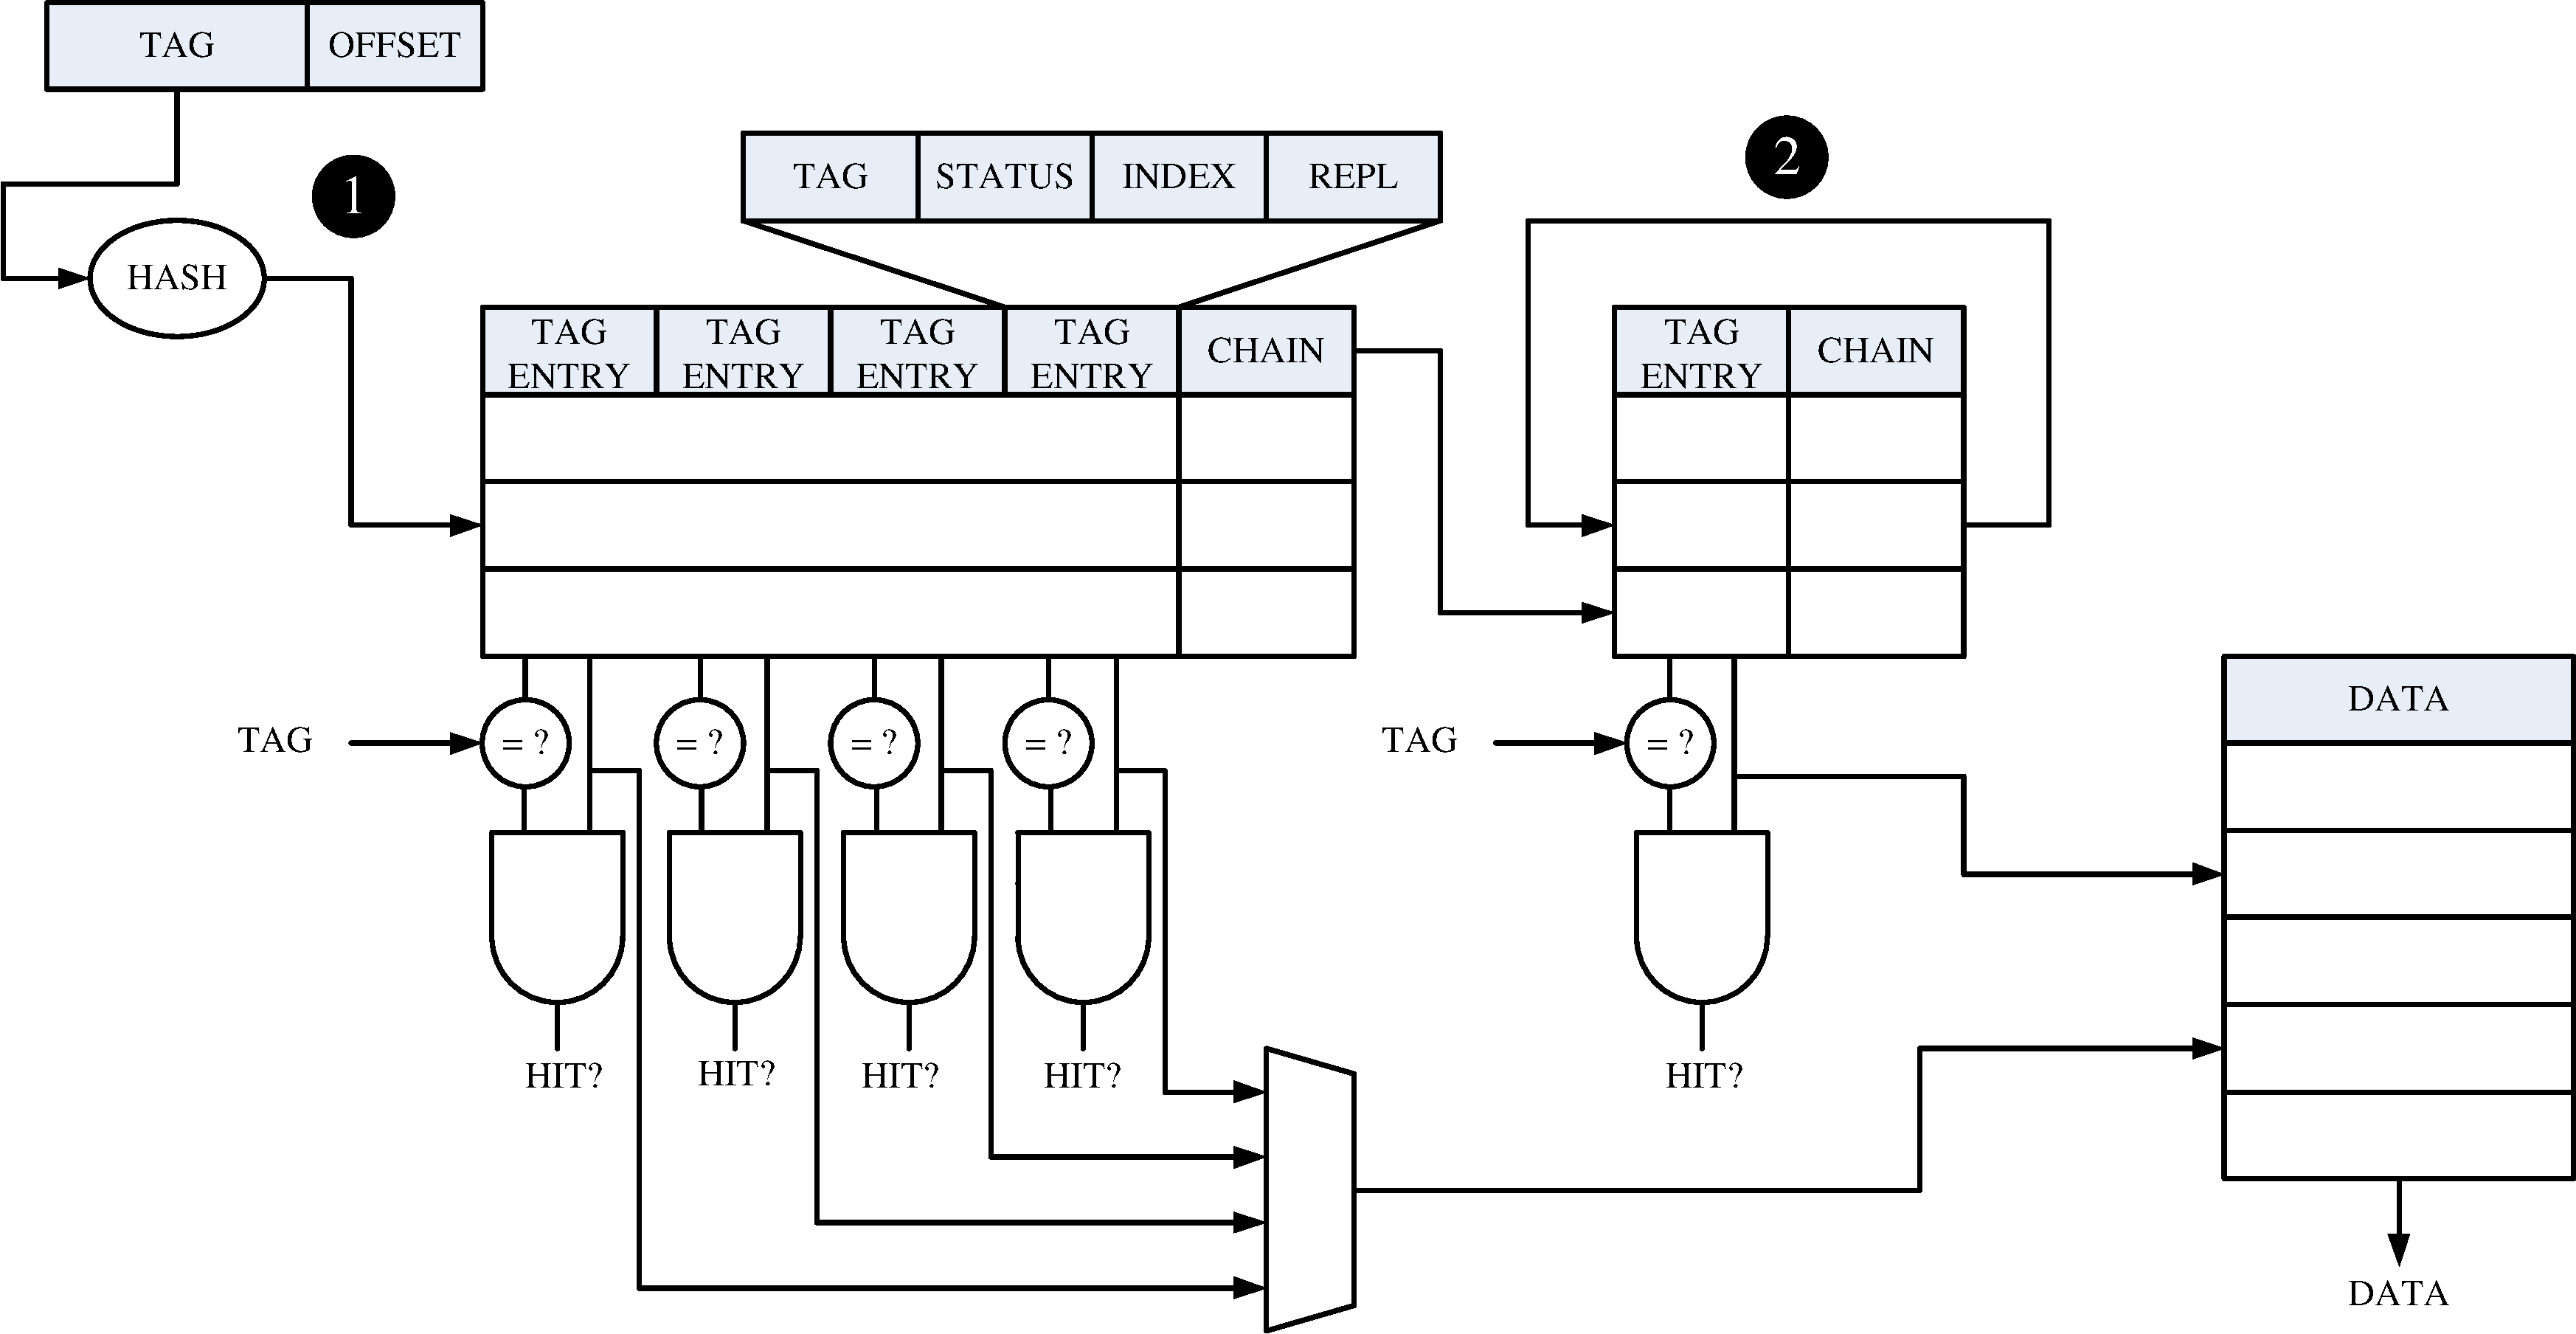
\includegraphics[width=\textwidth]{files/Figures/06-IIC.pdf}
  \\
  \caption[Indirect Index Cache]{\textbf{Indirect Index Cache} : The tag array for an IIC is split into two parts. A primary hash table and a secondary block for chaining. \bigspot{1} On each access, the block tag is hashed to obtain a primary table index. The primary table is associative, so a single search accesses the first few entries (4 in the example figure) of the hash chain. Collisions beyond this depth are chained into the secondary hash storage as shown in \bigspot{2}.}
  \label{fig:iic}
\end{figure}

In 2004, Hallnor et al\cite{Hallnor04acompressed} proposed a compressed memory hierarchy based on the IIC. Their design to support compression in the LLC was heavily inspired by IBM's Memory Expansion Technology(MXT)\cite{Pinnacle:2001}. The IIC already supported the random placement of blocks within a set with the index of the data block being stored in tag entry. With suitable modifications, the IIC was made to support compressed, variable granularity blocks. 

The IIC-Compressed design is similar to the \AC\ in the sense that it can cache variable granularity data blocks. However, the increased tag structure complexity and nature of serialised access to tags and data detract from its merits. The goals of caching variable granularity data blocks are different for the \AC{}(bandwidth and energy reduction) and the IIC(caching compressed blocks). 

\subsection{Other related work}

Recently Yoon et al. have proposed an adaptive granularity DRAM architecture\cite{Yoon_Jeong_Erez_2011}. This provides the support necessary for supporting variable granularity off-chip requests from an Amoeba-Cache-based LLC. Some research \cite{Dubnicki:1992:ABS:139669.139725,Choi:2011:DRM:2120965.2121416} has also focused on reducing false sharing in coherent caches by splitting/merging cache blocks to avoid invalidations. They would benefit from the Amoeba-Cache design, which manages block granularity in hardware. There has a been a significant amount of work at the compiler and software runtime level (e.g. \cite{Chilimbi-Hill-pldi-1999}) to restructure data for improved spatial efficiency. There have also been efforts from the architecture community to predict spatial locality \cite{pujara-hpca-2006, Watkins:2008:RCB:1505816.1505849, kumar-isca-1998, yoon2012dgms}, which we can leverage to predict Amoeba-Block ranges. Finally, cache compression is an orthogonal body of work that does not eliminate unused words but seeks to minimize the overall memory footprint \cite{AlameldeenPHD}.

